\documentclass[twoside]{book}

% Packages required by doxygen
\usepackage{calc}
\usepackage{doxygen}
\usepackage{graphicx}
\usepackage[utf8]{inputenc}
\usepackage{makeidx}
\usepackage{multicol}
\usepackage{multirow}
\usepackage{textcomp}
\usepackage[table]{xcolor}

% Font selection
\usepackage[T1]{fontenc}
\usepackage{mathptmx}
\usepackage[scaled=.90]{helvet}
\usepackage{courier}
\usepackage{amssymb}
\usepackage{sectsty}
\renewcommand{\familydefault}{\sfdefault}
\allsectionsfont{%
  \fontseries{bc}\selectfont%
  \color{darkgray}%
}
\renewcommand{\DoxyLabelFont}{%
  \fontseries{bc}\selectfont%
  \color{darkgray}%
}

% Page & text layout
\usepackage{geometry}
\geometry{%
  a4paper,%
  top=2.5cm,%
  bottom=2.5cm,%
  left=2.5cm,%
  right=2.5cm%
}
\tolerance=750
\hfuzz=15pt
\hbadness=750
\setlength{\emergencystretch}{15pt}
\setlength{\parindent}{0cm}
\setlength{\parskip}{0.2cm}
\makeatletter
\renewcommand{\paragraph}{%
  \@startsection{paragraph}{4}{0ex}{-1.0ex}{1.0ex}{%
    \normalfont\normalsize\bfseries\SS@parafont%
  }%
}
\renewcommand{\subparagraph}{%
  \@startsection{subparagraph}{5}{0ex}{-1.0ex}{1.0ex}{%
    \normalfont\normalsize\bfseries\SS@subparafont%
  }%
}
\makeatother

% Headers & footers
\usepackage{fancyhdr}
\pagestyle{fancyplain}
\fancyhead[LE]{\fancyplain{}{\bfseries\thepage}}
\fancyhead[CE]{\fancyplain{}{}}
\fancyhead[RE]{\fancyplain{}{\bfseries\leftmark}}
\fancyhead[LO]{\fancyplain{}{\bfseries\rightmark}}
\fancyhead[CO]{\fancyplain{}{}}
\fancyhead[RO]{\fancyplain{}{\bfseries\thepage}}
\fancyfoot[LE]{\fancyplain{}{}}
\fancyfoot[CE]{\fancyplain{}{}}
\fancyfoot[RE]{\fancyplain{}{\bfseries\scriptsize Generated on Tue Nov 28 2023 04\-:50\-:12 for Publisher by Doxygen }}
\fancyfoot[LO]{\fancyplain{}{\bfseries\scriptsize Generated on Tue Nov 28 2023 04\-:50\-:12 for Publisher by Doxygen }}
\fancyfoot[CO]{\fancyplain{}{}}
\fancyfoot[RO]{\fancyplain{}{}}
\renewcommand{\footrulewidth}{0.4pt}
\renewcommand{\chaptermark}[1]{%
  \markboth{#1}{}%
}
\renewcommand{\sectionmark}[1]{%
  \markright{\thesection\ #1}%
}

% Indices & bibliography
\usepackage{natbib}
\usepackage[titles]{tocloft}
\setcounter{tocdepth}{3}
\setcounter{secnumdepth}{5}
\makeindex

% Hyperlinks (required, but should be loaded last)
\usepackage{ifpdf}
\ifpdf
  \usepackage[pdftex,pagebackref=true]{hyperref}
\else
  \usepackage[ps2pdf,pagebackref=true]{hyperref}
\fi
\hypersetup{%
  colorlinks=true,%
  linkcolor=blue,%
  citecolor=blue,%
  unicode%
}

% Custom commands
\newcommand{\clearemptydoublepage}{%
  \newpage{\pagestyle{empty}\cleardoublepage}%
}


%===== C O N T E N T S =====

\begin{document}

% Titlepage & ToC
\hypersetup{pageanchor=false}
\pagenumbering{roman}
\begin{titlepage}
\vspace*{7cm}
\begin{center}%
{\Large Publisher }\\
\vspace*{1cm}
{\large Generated by Doxygen 1.8.5}\\
\vspace*{0.5cm}
{\small Tue Nov 28 2023 04:50:12}\\
\end{center}
\end{titlepage}
\clearemptydoublepage
\tableofcontents
\clearemptydoublepage
\pagenumbering{arabic}
\hypersetup{pageanchor=true}

%--- Begin generated contents ---
\chapter{Hierarchical Index}
\doxysection{Class Hierarchy}
This inheritance list is sorted roughly, but not completely, alphabetically\+:\begin{DoxyCompactList}
\item \contentsline{section}{Command\+Runner}{\pageref{classCommandRunner}}{}
\item \contentsline{section}{Data\+Buffer$<$ T $>$}{\pageref{classDataBuffer}}{}
\item \contentsline{section}{Data\+Buffer$<$ std\+::string $>$}{\pageref{classDataBuffer}}{}
\item \contentsline{section}{Data\+Channel}{\pageref{classDataChannel}}{}
\item \contentsline{section}{Data\+Channel\+Manager}{\pageref{classDataChannelManager}}{}
\item \contentsline{section}{Data\+Channel\+Processes\+Manager}{\pageref{classDataChannelProcessesManager}}{}
\item \contentsline{section}{Data\+Transmitter}{\pageref{classDataTransmitter}}{}
\item \contentsline{section}{Data\+Transmitter\+Manager}{\pageref{classDataTransmitterManager}}{}
\item \contentsline{section}{General\+Processor}{\pageref{classGeneralProcessor}}{}
\begin{DoxyCompactList}
\item \contentsline{section}{Command\+Processor}{\pageref{classCommandProcessor}}{}
\end{DoxyCompactList}
\item \contentsline{section}{General\+Processor\+Factory}{\pageref{classGeneralProcessorFactory}}{}
\item \contentsline{section}{Json\+Manager}{\pageref{classJsonManager}}{}
\item \contentsline{section}{Project\+Printer}{\pageref{classProjectPrinter}}{}
\item \contentsline{section}{Signal\+Handler}{\pageref{classSignalHandler}}{}
\item \contentsline{section}{Type\+Checker}{\pageref{classTypeChecker}}{}
\end{DoxyCompactList}

\chapter{Class Index}
\section{Class List}
Here are the classes, structs, unions and interfaces with brief descriptions\-:\begin{DoxyCompactList}
\item\contentsline{section}{\hyperlink{classCommandProcessor}{Command\-Processor} }{\pageref{classCommandProcessor}}{}
\item\contentsline{section}{\hyperlink{classCommandRunner}{Command\-Runner} }{\pageref{classCommandRunner}}{}
\item\contentsline{section}{\hyperlink{classDataBuffer}{Data\-Buffer$<$ T $>$} }{\pageref{classDataBuffer}}{}
\item\contentsline{section}{\hyperlink{classDataChannel}{Data\-Channel} }{\pageref{classDataChannel}}{}
\item\contentsline{section}{\hyperlink{classDataChannelManager}{Data\-Channel\-Manager} }{\pageref{classDataChannelManager}}{}
\item\contentsline{section}{\hyperlink{classDataChannelProcessesManager}{Data\-Channel\-Processes\-Manager} }{\pageref{classDataChannelProcessesManager}}{}
\item\contentsline{section}{\hyperlink{classDataTransmitter}{Data\-Transmitter} }{\pageref{classDataTransmitter}}{}
\item\contentsline{section}{\hyperlink{classDataTransmitterManager}{Data\-Transmitter\-Manager} }{\pageref{classDataTransmitterManager}}{}
\item\contentsline{section}{\hyperlink{classEventLoopManager}{Event\-Loop\-Manager} }{\pageref{classEventLoopManager}}{}
\item\contentsline{section}{\hyperlink{classGeneralProcessor}{General\-Processor} }{\pageref{classGeneralProcessor}}{}
\item\contentsline{section}{\hyperlink{classGeneralProcessorFactory}{General\-Processor\-Factory} }{\pageref{classGeneralProcessorFactory}}{}
\item\contentsline{section}{\hyperlink{classJsonManager}{Json\-Manager} }{\pageref{classJsonManager}}{}
\item\contentsline{section}{\hyperlink{classProjectPrinter}{Project\-Printer} }{\pageref{classProjectPrinter}}{}
\item\contentsline{section}{\hyperlink{classSignalHandler}{Signal\-Handler} }{\pageref{classSignalHandler}}{}
\item\contentsline{section}{\hyperlink{classTypeChecker}{Type\-Checker} }{\pageref{classTypeChecker}}{}
\end{DoxyCompactList}

\chapter{File Index}
\section{File List}
Here is a list of all documented files with brief descriptions\-:\begin{DoxyCompactList}
\item\contentsline{section}{\hyperlink{main_8cpp}{main.\-cpp} \\*Entry point for the program }{\pageref{main_8cpp}}{}
\item\contentsline{section}{command\-\_\-management/{\bfseries Command\-Runner.\-h} }{\pageref{CommandRunner_8h}}{}
\item\contentsline{section}{data\-\_\-transmitter/{\bfseries Data\-Buffer.\-h} }{\pageref{DataBuffer_8h}}{}
\item\contentsline{section}{data\-\_\-transmitter/{\bfseries Data\-Channel.\-h} }{\pageref{DataChannel_8h}}{}
\item\contentsline{section}{data\-\_\-transmitter/{\bfseries Data\-Channel\-Manager.\-h} }{\pageref{DataChannelManager_8h}}{}
\item\contentsline{section}{data\-\_\-transmitter/{\bfseries Data\-Channel\-Processes\-Manager.\-h} }{\pageref{DataChannelProcessesManager_8h}}{}
\item\contentsline{section}{data\-\_\-transmitter/{\bfseries Data\-Transmitter.\-h} }{\pageref{DataTransmitter_8h}}{}
\item\contentsline{section}{data\-\_\-transmitter/{\bfseries Data\-Transmitter\-Manager.\-h} }{\pageref{DataTransmitterManager_8h}}{}
\item\contentsline{section}{processors/{\bfseries Command\-Processor.\-h} }{\pageref{CommandProcessor_8h}}{}
\item\contentsline{section}{processors/{\bfseries General\-Processor.\-h} }{\pageref{GeneralProcessor_8h}}{}
\item\contentsline{section}{processors/{\bfseries General\-Processor\-Factory.\-h} }{\pageref{GeneralProcessorFactory_8h}}{}
\item\contentsline{section}{utilities/{\bfseries Event\-Loop\-Manager.\-h} }{\pageref{EventLoopManager_8h}}{}
\item\contentsline{section}{utilities/{\bfseries Json\-Manager.\-h} }{\pageref{JsonManager_8h}}{}
\item\contentsline{section}{utilities/{\bfseries Project\-Printer.\-h} }{\pageref{ProjectPrinter_8h}}{}
\item\contentsline{section}{utilities/{\bfseries Signal\-Handler.\-h} }{\pageref{SignalHandler_8h}}{}
\item\contentsline{section}{utilities/{\bfseries Type\-Checker.\-h} }{\pageref{TypeChecker_8h}}{}
\end{DoxyCompactList}

\chapter{Class Documentation}
\hypertarget{classCommandProcessor}{}\doxysection{Command\+Processor Class Reference}
\label{classCommandProcessor}\index{CommandProcessor@{CommandProcessor}}


A processor that executes commands and processes their output.  




{\ttfamily \#include $<$Command\+Processor.\+h$>$}

Inheritance diagram for Command\+Processor\+:\begin{figure}[H]
\begin{center}
\leavevmode
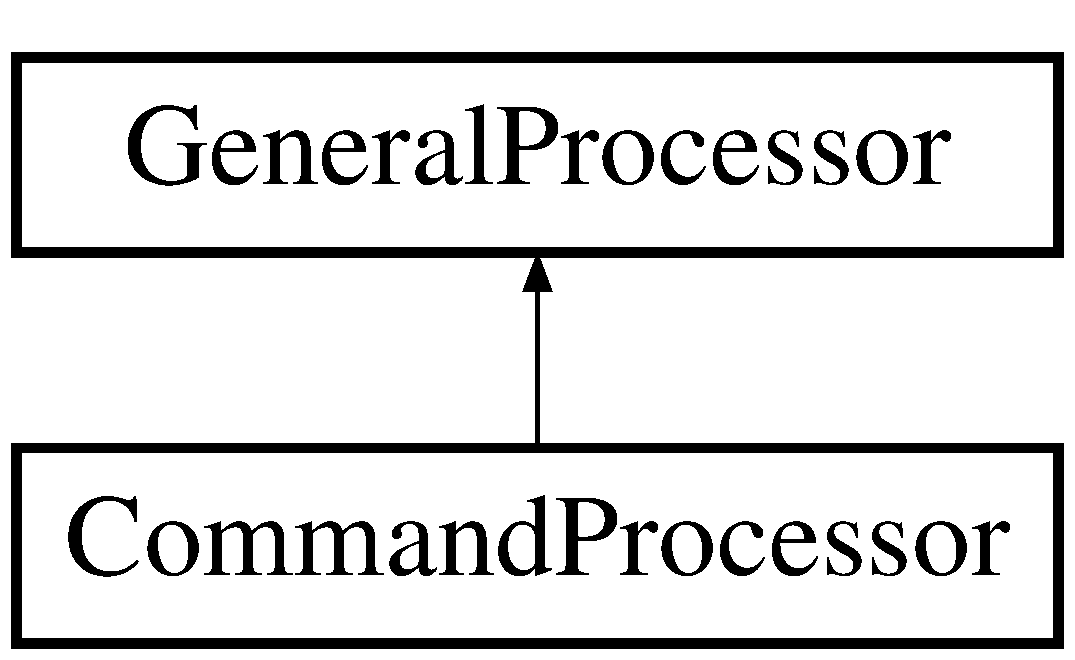
\includegraphics[height=2.000000cm]{classCommandProcessor}
\end{center}
\end{figure}
\doxysubsection*{Public Member Functions}
\begin{DoxyCompactItemize}
\item 
\mbox{\hyperlink{classCommandProcessor_a8efe4696ca63e76dfabe66a5e1ae975c}{Command\+Processor}} (int \mbox{\hyperlink{classGeneralProcessor_ade0b12d7fec2b58a9782559734b00012}{verbose}}=0, const \mbox{\hyperlink{classCommandRunner}{Command\+Runner}} \&runner=\mbox{\hyperlink{classCommandRunner}{Command\+Runner}}(\char`\"{}\char`\"{}))
\begin{DoxyCompactList}\small\item\em Constructor for \mbox{\hyperlink{classCommandProcessor}{Command\+Processor}}. \end{DoxyCompactList}\item 
\mbox{\Hypertarget{classCommandProcessor_a567d3d2e76bcfa2b8780dca68e74d641}\label{classCommandProcessor_a567d3d2e76bcfa2b8780dca68e74d641}} 
\mbox{\hyperlink{classCommandProcessor_a567d3d2e76bcfa2b8780dca68e74d641}{$\sim$\+Command\+Processor}} () override
\begin{DoxyCompactList}\small\item\em Destructor for \mbox{\hyperlink{classCommandProcessor}{Command\+Processor}}. \end{DoxyCompactList}\item 
std\+::vector$<$ std\+::string $>$ \mbox{\hyperlink{classCommandProcessor_ae1415f17b13b6017839e1dff5c384e2c}{get\+Processed\+Output}} () override
\begin{DoxyCompactList}\small\item\em Gets the processed output after executing the command. \end{DoxyCompactList}\item 
virtual void \mbox{\hyperlink{classCommandProcessor_af344f7b0c5ee1bf8b6f675135ff0a7c5}{set\+Command\+Runner}} (const \mbox{\hyperlink{classCommandRunner}{Command\+Runner}} \&runner)
\begin{DoxyCompactList}\small\item\em Sets the command runner for executing commands. \end{DoxyCompactList}\item 
const \mbox{\hyperlink{classCommandRunner}{Command\+Runner}} \& \mbox{\hyperlink{classCommandProcessor_ad0beedad9b0535415eaf8762dbc32d34}{get\+Command\+Runner}} () const
\begin{DoxyCompactList}\small\item\em Gets the current command runner. \end{DoxyCompactList}\item 
bool \mbox{\hyperlink{classCommandProcessor_ae1b2f30c9de7dcfad246f4612afe7bb8}{is\+Ready\+To\+Process}} () const override
\begin{DoxyCompactList}\small\item\em Checks if the processor is ready to process. \end{DoxyCompactList}\item 
int \mbox{\hyperlink{classCommandProcessor_abb5a1f0942b285a0ae06b6cbce225621}{get\+Period}} () const override
\begin{DoxyCompactList}\small\item\em Gets the processing period for the \mbox{\hyperlink{classCommandProcessor}{Command\+Processor}}. \end{DoxyCompactList}\item 
void \mbox{\hyperlink{classCommandProcessor_a6366c78835ecc66e0dcfa3094a194de2}{set\+Period}} (int new\+Period) override
\begin{DoxyCompactList}\small\item\em Sets the processing period for the \mbox{\hyperlink{classCommandProcessor}{Command\+Processor}}. \end{DoxyCompactList}\end{DoxyCompactItemize}
\doxysubsection*{Protected Attributes}
\begin{DoxyCompactItemize}
\item 
\mbox{\Hypertarget{classCommandProcessor_a136f0b6c6c6133675ce7aa22d582128e}\label{classCommandProcessor_a136f0b6c6c6133675ce7aa22d582128e}} 
\mbox{\hyperlink{classCommandRunner}{Command\+Runner}} \mbox{\hyperlink{classCommandProcessor_a136f0b6c6c6133675ce7aa22d582128e}{command\+Runner}}
\begin{DoxyCompactList}\small\item\em The command runner responsible for executing commands. \end{DoxyCompactList}\end{DoxyCompactItemize}


\doxysubsection{Detailed Description}
A processor that executes commands and processes their output. 

The {\ttfamily \mbox{\hyperlink{classCommandProcessor}{Command\+Processor}}} class is a specialization of {\ttfamily \mbox{\hyperlink{classGeneralProcessor}{General\+Processor}}} that executes commands using a {\ttfamily \mbox{\hyperlink{classCommandRunner}{Command\+Runner}}} and processes the command output. 

\doxysubsection{Constructor \& Destructor Documentation}
\mbox{\Hypertarget{classCommandProcessor_a8efe4696ca63e76dfabe66a5e1ae975c}\label{classCommandProcessor_a8efe4696ca63e76dfabe66a5e1ae975c}} 
\index{CommandProcessor@{CommandProcessor}!CommandProcessor@{CommandProcessor}}
\index{CommandProcessor@{CommandProcessor}!CommandProcessor@{CommandProcessor}}
\doxysubsubsection{\texorpdfstring{CommandProcessor()}{CommandProcessor()}}
{\footnotesize\ttfamily Command\+Processor\+::\+Command\+Processor (\begin{DoxyParamCaption}\item[{int}]{verbose = {\ttfamily 0},  }\item[{const \mbox{\hyperlink{classCommandRunner}{Command\+Runner}} \&}]{runner = {\ttfamily \mbox{\hyperlink{classCommandRunner}{Command\+Runner}}(\char`\"{}\char`\"{})} }\end{DoxyParamCaption})}



Constructor for \mbox{\hyperlink{classCommandProcessor}{Command\+Processor}}. 


\begin{DoxyParams}{Parameters}
{\em verbose} & The verbosity level for logging (default is 0). \\
\hline
{\em runner} & The command runner responsible for executing commands (default is an empty runner). \\
\hline
\end{DoxyParams}


\doxysubsection{Member Function Documentation}
\mbox{\Hypertarget{classCommandProcessor_ad0beedad9b0535415eaf8762dbc32d34}\label{classCommandProcessor_ad0beedad9b0535415eaf8762dbc32d34}} 
\index{CommandProcessor@{CommandProcessor}!getCommandRunner@{getCommandRunner}}
\index{getCommandRunner@{getCommandRunner}!CommandProcessor@{CommandProcessor}}
\doxysubsubsection{\texorpdfstring{getCommandRunner()}{getCommandRunner()}}
{\footnotesize\ttfamily const \mbox{\hyperlink{classCommandRunner}{Command\+Runner}} \& Command\+Processor\+::get\+Command\+Runner (\begin{DoxyParamCaption}{ }\end{DoxyParamCaption}) const}



Gets the current command runner. 

\begin{DoxyReturn}{Returns}
Reference to the current command runner. 
\end{DoxyReturn}
\mbox{\Hypertarget{classCommandProcessor_abb5a1f0942b285a0ae06b6cbce225621}\label{classCommandProcessor_abb5a1f0942b285a0ae06b6cbce225621}} 
\index{CommandProcessor@{CommandProcessor}!getPeriod@{getPeriod}}
\index{getPeriod@{getPeriod}!CommandProcessor@{CommandProcessor}}
\doxysubsubsection{\texorpdfstring{getPeriod()}{getPeriod()}}
{\footnotesize\ttfamily int Command\+Processor\+::get\+Period (\begin{DoxyParamCaption}{ }\end{DoxyParamCaption}) const\hspace{0.3cm}{\ttfamily [override]}, {\ttfamily [virtual]}}



Gets the processing period for the \mbox{\hyperlink{classCommandProcessor}{Command\+Processor}}. 

\begin{DoxyReturn}{Returns}
The processing period. 
\end{DoxyReturn}


Reimplemented from \mbox{\hyperlink{classGeneralProcessor_a8d3433cced851b340d3a2b41bc031a32}{General\+Processor}}.

\mbox{\Hypertarget{classCommandProcessor_ae1415f17b13b6017839e1dff5c384e2c}\label{classCommandProcessor_ae1415f17b13b6017839e1dff5c384e2c}} 
\index{CommandProcessor@{CommandProcessor}!getProcessedOutput@{getProcessedOutput}}
\index{getProcessedOutput@{getProcessedOutput}!CommandProcessor@{CommandProcessor}}
\doxysubsubsection{\texorpdfstring{getProcessedOutput()}{getProcessedOutput()}}
{\footnotesize\ttfamily std\+::vector$<$ std\+::string $>$ Command\+Processor\+::get\+Processed\+Output (\begin{DoxyParamCaption}{ }\end{DoxyParamCaption})\hspace{0.3cm}{\ttfamily [override]}, {\ttfamily [virtual]}}



Gets the processed output after executing the command. 

\begin{DoxyReturn}{Returns}
Vector of strings representing the processed output. 
\end{DoxyReturn}


Reimplemented from \mbox{\hyperlink{classGeneralProcessor_ac25327015ff4e08b1b195e08ca5c551e}{General\+Processor}}.

\mbox{\Hypertarget{classCommandProcessor_ae1b2f30c9de7dcfad246f4612afe7bb8}\label{classCommandProcessor_ae1b2f30c9de7dcfad246f4612afe7bb8}} 
\index{CommandProcessor@{CommandProcessor}!isReadyToProcess@{isReadyToProcess}}
\index{isReadyToProcess@{isReadyToProcess}!CommandProcessor@{CommandProcessor}}
\doxysubsubsection{\texorpdfstring{isReadyToProcess()}{isReadyToProcess()}}
{\footnotesize\ttfamily bool Command\+Processor\+::is\+Ready\+To\+Process (\begin{DoxyParamCaption}{ }\end{DoxyParamCaption}) const\hspace{0.3cm}{\ttfamily [override]}, {\ttfamily [virtual]}}



Checks if the processor is ready to process. 

\begin{DoxyReturn}{Returns}
True if ready to process, false otherwise. 
\end{DoxyReturn}


Reimplemented from \mbox{\hyperlink{classGeneralProcessor_ac6795bb2b996d8e5b09ed998a553c8e5}{General\+Processor}}.

\mbox{\Hypertarget{classCommandProcessor_af344f7b0c5ee1bf8b6f675135ff0a7c5}\label{classCommandProcessor_af344f7b0c5ee1bf8b6f675135ff0a7c5}} 
\index{CommandProcessor@{CommandProcessor}!setCommandRunner@{setCommandRunner}}
\index{setCommandRunner@{setCommandRunner}!CommandProcessor@{CommandProcessor}}
\doxysubsubsection{\texorpdfstring{setCommandRunner()}{setCommandRunner()}}
{\footnotesize\ttfamily void Command\+Processor\+::set\+Command\+Runner (\begin{DoxyParamCaption}\item[{const \mbox{\hyperlink{classCommandRunner}{Command\+Runner}} \&}]{runner }\end{DoxyParamCaption})\hspace{0.3cm}{\ttfamily [virtual]}}



Sets the command runner for executing commands. 


\begin{DoxyParams}{Parameters}
{\em runner} & The command runner to set.\\
\hline
\end{DoxyParams}
The command runner class gets automatically generated and set based on the config. \begin{DoxySeeAlso}{See also}
\mbox{\hyperlink{classDataChannelManager_aacbb944add821588a735a0516888b931}{Data\+Channel\+Manager\+::add\+Channel}} 
\end{DoxySeeAlso}
\mbox{\Hypertarget{classCommandProcessor_a6366c78835ecc66e0dcfa3094a194de2}\label{classCommandProcessor_a6366c78835ecc66e0dcfa3094a194de2}} 
\index{CommandProcessor@{CommandProcessor}!setPeriod@{setPeriod}}
\index{setPeriod@{setPeriod}!CommandProcessor@{CommandProcessor}}
\doxysubsubsection{\texorpdfstring{setPeriod()}{setPeriod()}}
{\footnotesize\ttfamily void Command\+Processor\+::set\+Period (\begin{DoxyParamCaption}\item[{int}]{new\+Period }\end{DoxyParamCaption})\hspace{0.3cm}{\ttfamily [override]}, {\ttfamily [virtual]}}



Sets the processing period for the \mbox{\hyperlink{classCommandProcessor}{Command\+Processor}}. 


\begin{DoxyParams}{Parameters}
{\em new\+Period} & The new processing period. \\
\hline
\end{DoxyParams}


Reimplemented from \mbox{\hyperlink{classGeneralProcessor_ae57c2ab2c7cc2a67fd535d388c39e3de}{General\+Processor}}.



The documentation for this class was generated from the following files\+:\begin{DoxyCompactItemize}
\item 
processors/Command\+Processor.\+h\item 
processors/Command\+Processor.\+cpp\end{DoxyCompactItemize}

\hypertarget{classCommandRunner}{\section{Command\-Runner Class Reference}
\label{classCommandRunner}\index{Command\-Runner@{Command\-Runner}}
}
\subsection*{Public Member Functions}
\begin{DoxyCompactItemize}
\item 
\hypertarget{classCommandRunner_a9e642e4704b083084100ded9357e098a}{{\bfseries Command\-Runner} (const std\-::string \&command)}\label{classCommandRunner_a9e642e4704b083084100ded9357e098a}

\item 
\hypertarget{classCommandRunner_a253f130e48e007bfef6160e4907f25a9}{{\bfseries Command\-Runner} (const std\-::vector$<$ std\-::string $>$ \&command\-With\-Args)}\label{classCommandRunner_a253f130e48e007bfef6160e4907f25a9}

\item 
\hypertarget{classCommandRunner_aa9f4aec533d160749766ae4d27b5fca5}{void {\bfseries add\-Argument} (const std\-::string \&arg)}\label{classCommandRunner_aa9f4aec533d160749766ae4d27b5fca5}

\item 
\hypertarget{classCommandRunner_a962a39f1d12393211becfbf7f0ae123f}{void {\bfseries set\-Wait\-Time} (int milliseconds)}\label{classCommandRunner_a962a39f1d12393211becfbf7f0ae123f}

\item 
\hypertarget{classCommandRunner_a75a0a138a720cf56f94409f78891c4b0}{std\-::string {\bfseries execute} ()}\label{classCommandRunner_a75a0a138a720cf56f94409f78891c4b0}

\item 
\hypertarget{classCommandRunner_a6e22a52434faa6cc419ae26e539006b7}{bool {\bfseries is\-Ready\-For\-Execution} () const }\label{classCommandRunner_a6e22a52434faa6cc419ae26e539006b7}

\item 
\hypertarget{classCommandRunner_ade72368d3f9f783fc3535d992491ad97}{std\-::string {\bfseries get\-Command} () const }\label{classCommandRunner_ade72368d3f9f783fc3535d992491ad97}

\item 
\hypertarget{classCommandRunner_afab3f2ed4515ce903fc489c16d07bf5b}{int {\bfseries get\-Wait\-Time} () const }\label{classCommandRunner_afab3f2ed4515ce903fc489c16d07bf5b}

\end{DoxyCompactItemize}
\subsection*{Protected Attributes}
\begin{DoxyCompactItemize}
\item 
\hypertarget{classCommandRunner_a698a3db746e478a8f8473aefba861c12}{std\-::vector$<$ std\-::string $>$ {\bfseries command\-With\-Args\-\_\-}}\label{classCommandRunner_a698a3db746e478a8f8473aefba861c12}

\item 
\hypertarget{classCommandRunner_a9e1bf64d642a722eea30601df75fac2a}{int {\bfseries wait\-Time\-\_\-}}\label{classCommandRunner_a9e1bf64d642a722eea30601df75fac2a}

\item 
\hypertarget{classCommandRunner_a13fbe69bf315d3016b7dbcc75b71247b}{std\-::chrono\-::time\-\_\-point\\*
$<$ std\-::chrono\-::high\-\_\-resolution\-\_\-clock $>$ {\bfseries last\-Execution\-Time}}\label{classCommandRunner_a13fbe69bf315d3016b7dbcc75b71247b}

\end{DoxyCompactItemize}


The documentation for this class was generated from the following files\-:\begin{DoxyCompactItemize}
\item 
command\-\_\-management/Command\-Runner.\-h\item 
command\-\_\-management/Command\-Runner.\-cpp\end{DoxyCompactItemize}

\hypertarget{classDataBuffer}{}\doxysection{Data\+Buffer$<$ T $>$ Class Template Reference}
\label{classDataBuffer}\index{DataBuffer$<$ T $>$@{DataBuffer$<$ T $>$}}


A circular buffer for storing data of a specified type.  




{\ttfamily \#include $<$Data\+Buffer.\+h$>$}

\doxysubsection*{Public Member Functions}
\begin{DoxyCompactItemize}
\item 
\mbox{\hyperlink{classDataBuffer_aa51e4cb7147b6d341aff27f247ff867a}{Data\+Buffer}} (size\+\_\+t size)
\begin{DoxyCompactList}\small\item\em Constructor for \mbox{\hyperlink{classDataBuffer}{Data\+Buffer}} with a specified size. \end{DoxyCompactList}\item 
void \mbox{\hyperlink{classDataBuffer_ac416fee4f7f5708cd747baa091701631}{Push}} (const T \&data)
\begin{DoxyCompactList}\small\item\em Pushes new data into the circular buffer. \end{DoxyCompactList}\item 
std\+::vector$<$ T $>$ \mbox{\hyperlink{classDataBuffer_a53a58dfc588df74ea9484dae7e7a3471}{Get\+Buffer}} () const
\begin{DoxyCompactList}\small\item\em Gets the buffer content as a vector. \end{DoxyCompactList}\item 
std\+::string \mbox{\hyperlink{classDataBuffer_ab7df68f0442748698eb180d480c050f3}{Serialize\+Buffer}} () const
\begin{DoxyCompactList}\small\item\em Serializes the buffer content to a JSON string. \end{DoxyCompactList}\end{DoxyCompactItemize}


\doxysubsection{Detailed Description}
\subsubsection*{template$<$typename T$>$\newline
class Data\+Buffer$<$ T $>$}

A circular buffer for storing data of a specified type. 

The {\ttfamily \mbox{\hyperlink{classDataBuffer}{Data\+Buffer}}} class implements a circular buffer to store data of a specified type. It allows pushing new data into the buffer and provides methods to retrieve and serialize the buffered data.


\begin{DoxyTemplParams}{Template Parameters}
{\em T} & The type of data to be stored in the buffer. \\
\hline
\end{DoxyTemplParams}


\doxysubsection{Constructor \& Destructor Documentation}
\mbox{\Hypertarget{classDataBuffer_aa51e4cb7147b6d341aff27f247ff867a}\label{classDataBuffer_aa51e4cb7147b6d341aff27f247ff867a}} 
\index{DataBuffer$<$ T $>$@{DataBuffer$<$ T $>$}!DataBuffer@{DataBuffer}}
\index{DataBuffer@{DataBuffer}!DataBuffer$<$ T $>$@{DataBuffer$<$ T $>$}}
\doxysubsubsection{\texorpdfstring{DataBuffer()}{DataBuffer()}}
{\footnotesize\ttfamily template$<$typename T $>$ \\
\mbox{\hyperlink{classDataBuffer}{Data\+Buffer}}$<$ T $>$\+::\mbox{\hyperlink{classDataBuffer}{Data\+Buffer}} (\begin{DoxyParamCaption}\item[{size\+\_\+t}]{size }\end{DoxyParamCaption})\hspace{0.3cm}{\ttfamily [inline]}}



Constructor for \mbox{\hyperlink{classDataBuffer}{Data\+Buffer}} with a specified size. 


\begin{DoxyParams}{Parameters}
{\em size} & The size of the circular buffer. \\
\hline
\end{DoxyParams}


\doxysubsection{Member Function Documentation}
\mbox{\Hypertarget{classDataBuffer_a53a58dfc588df74ea9484dae7e7a3471}\label{classDataBuffer_a53a58dfc588df74ea9484dae7e7a3471}} 
\index{DataBuffer$<$ T $>$@{DataBuffer$<$ T $>$}!GetBuffer@{GetBuffer}}
\index{GetBuffer@{GetBuffer}!DataBuffer$<$ T $>$@{DataBuffer$<$ T $>$}}
\doxysubsubsection{\texorpdfstring{GetBuffer()}{GetBuffer()}}
{\footnotesize\ttfamily template$<$typename T $>$ \\
std\+::vector$<$T$>$ \mbox{\hyperlink{classDataBuffer}{Data\+Buffer}}$<$ T $>$\+::Get\+Buffer (\begin{DoxyParamCaption}{ }\end{DoxyParamCaption}) const\hspace{0.3cm}{\ttfamily [inline]}}



Gets the buffer content as a vector. 

\begin{DoxyReturn}{Returns}
A vector containing the buffered data. 
\end{DoxyReturn}
\mbox{\Hypertarget{classDataBuffer_ac416fee4f7f5708cd747baa091701631}\label{classDataBuffer_ac416fee4f7f5708cd747baa091701631}} 
\index{DataBuffer$<$ T $>$@{DataBuffer$<$ T $>$}!Push@{Push}}
\index{Push@{Push}!DataBuffer$<$ T $>$@{DataBuffer$<$ T $>$}}
\doxysubsubsection{\texorpdfstring{Push()}{Push()}}
{\footnotesize\ttfamily template$<$typename T $>$ \\
void \mbox{\hyperlink{classDataBuffer}{Data\+Buffer}}$<$ T $>$\+::Push (\begin{DoxyParamCaption}\item[{const T \&}]{data }\end{DoxyParamCaption})\hspace{0.3cm}{\ttfamily [inline]}}



Pushes new data into the circular buffer. 


\begin{DoxyParams}{Parameters}
{\em data} & The data to be pushed into the buffer. \\
\hline
\end{DoxyParams}
\mbox{\Hypertarget{classDataBuffer_ab7df68f0442748698eb180d480c050f3}\label{classDataBuffer_ab7df68f0442748698eb180d480c050f3}} 
\index{DataBuffer$<$ T $>$@{DataBuffer$<$ T $>$}!SerializeBuffer@{SerializeBuffer}}
\index{SerializeBuffer@{SerializeBuffer}!DataBuffer$<$ T $>$@{DataBuffer$<$ T $>$}}
\doxysubsubsection{\texorpdfstring{SerializeBuffer()}{SerializeBuffer()}}
{\footnotesize\ttfamily template$<$typename T $>$ \\
std\+::string \mbox{\hyperlink{classDataBuffer}{Data\+Buffer}}$<$ T $>$\+::Serialize\+Buffer (\begin{DoxyParamCaption}{ }\end{DoxyParamCaption}) const\hspace{0.3cm}{\ttfamily [inline]}}



Serializes the buffer content to a JSON string. 

\begin{DoxyReturn}{Returns}
A JSON string representing the buffered data. 
\end{DoxyReturn}


The documentation for this class was generated from the following file\+:\begin{DoxyCompactItemize}
\item 
data\+\_\+transmitter/Data\+Buffer.\+h\end{DoxyCompactItemize}

\hypertarget{classDataChannel}{}\doxysection{Data\+Channel Class Reference}
\label{classDataChannel}\index{DataChannel@{DataChannel}}


Represents a data channel for publishing events.  




{\ttfamily \#include $<$Data\+Channel.\+h$>$}

\doxysubsection*{Public Member Functions}
\begin{DoxyCompactItemize}
\item 
\mbox{\Hypertarget{classDataChannel_a44413122b5ae4f88340adee334dd392e}\label{classDataChannel_a44413122b5ae4f88340adee334dd392e}} 
\mbox{\hyperlink{classDataChannel_a44413122b5ae4f88340adee334dd392e}{Data\+Channel}} ()
\begin{DoxyCompactList}\small\item\em Default constructor for \mbox{\hyperlink{classDataChannel}{Data\+Channel}}. \end{DoxyCompactList}\item 
\mbox{\hyperlink{classDataChannel_afddd4706fd837ed68f509425bc3a6b66}{Data\+Channel}} (const std\+::string \&name, int events\+Before\+Break, int events\+To\+Ignore\+In\+Break)
\begin{DoxyCompactList}\small\item\em Constructor for \mbox{\hyperlink{classDataChannel}{Data\+Channel}} with specified attributes. \end{DoxyCompactList}\item 
\mbox{\hyperlink{classDataChannel_aede3c0b8afa801ffd300d65fb91e9fdd}{Data\+Channel}} (const std\+::string \&name, int events\+Before\+Break, int events\+To\+Ignore\+In\+Break, const std\+::string \&address)
\begin{DoxyCompactList}\small\item\em Constructor for \mbox{\hyperlink{classDataChannel}{Data\+Channel}} with specified attributes and address. \end{DoxyCompactList}\item 
bool \mbox{\hyperlink{classDataChannel_ab9e138d3332e8c540bb1769c4dab8517}{publish}} ()
\begin{DoxyCompactList}\small\item\em Publishes events for the data channel. \end{DoxyCompactList}\item 
void \mbox{\hyperlink{classDataChannel_ab5f6bc6ce5d7f83a26598069df067c5f}{set\+Name}} (const std\+::string \&name)
\begin{DoxyCompactList}\small\item\em Sets the name of the data channel. \end{DoxyCompactList}\item 
void \mbox{\hyperlink{classDataChannel_a640900fcffff28e003bc0a34e6d4d68a}{set\+Events\+Before\+Break}} (int events\+Before\+Break)
\begin{DoxyCompactList}\small\item\em Sets the number of events before taking a break. \end{DoxyCompactList}\item 
void \mbox{\hyperlink{classDataChannel_ab7faf42f153cdae64b36ed8f0f723dca}{set\+Events\+To\+Ignore\+In\+Break}} (int events\+To\+Ignore\+In\+Break)
\begin{DoxyCompactList}\small\item\em Sets the number of events to ignore during a break. \end{DoxyCompactList}\item 
void \mbox{\hyperlink{classDataChannel_a293e391e94c5920151a531078ecf9891}{set\+Address}} (const std\+::string \&address)
\begin{DoxyCompactList}\small\item\em Sets the address associated with the data channel. \end{DoxyCompactList}\item 
const std\+::string \& \mbox{\hyperlink{classDataChannel_aec020d154f233b2873708a3123378040}{get\+Name}} () const
\begin{DoxyCompactList}\small\item\em Gets the name of the data channel. \end{DoxyCompactList}\item 
int \mbox{\hyperlink{classDataChannel_ad42b27120b73d4a5fe17acc52269d37a}{get\+Events\+Before\+Break}} () const
\begin{DoxyCompactList}\small\item\em Gets the number of events before taking a break. \end{DoxyCompactList}\item 
int \mbox{\hyperlink{classDataChannel_a6f8981227b1c9345847aa0a8d715b072}{get\+Events\+To\+Ignore\+In\+Break}} () const
\begin{DoxyCompactList}\small\item\em Gets the number of events to ignore during a break. \end{DoxyCompactList}\item 
const std\+::string \& \mbox{\hyperlink{classDataChannel_ae2b355c0cc2684c35257bcee6b8a9ba5}{get\+Address}} () const
\begin{DoxyCompactList}\small\item\em Gets the address associated with the data channel. \end{DoxyCompactList}\item 
int \mbox{\hyperlink{classDataChannel_a940ce0e07433910d1648a7eab5151903}{get\+Events\+Published}} () const
\begin{DoxyCompactList}\small\item\em Gets the number of events published. \end{DoxyCompactList}\item 
int \mbox{\hyperlink{classDataChannel_a49b993d93406299654b8707ecbbcc867}{get\+Events\+Seen}} () const
\begin{DoxyCompactList}\small\item\em Gets the number of events seen. \end{DoxyCompactList}\item 
bool \mbox{\hyperlink{classDataChannel_ac6b307906f4ea74ec5774fb5a5cfe98d}{is\+On\+Break}} () const
\begin{DoxyCompactList}\small\item\em Checks if the data channel is on break. \end{DoxyCompactList}\item 
int \mbox{\hyperlink{classDataChannel_a0e58d89fd9f8a7b21c25f10c6ef3b70e}{get\+Events\+Seen\+On\+Break}} () const
\begin{DoxyCompactList}\small\item\em Gets the number of events seen during a break. \end{DoxyCompactList}\item 
int \mbox{\hyperlink{classDataChannel_a1b3c25b7bd5a39cf1d5c0cf73954e307}{get\+Tick\+Time}} () const
\begin{DoxyCompactList}\small\item\em Gets the tick time for the data channel. \end{DoxyCompactList}\item 
\mbox{\Hypertarget{classDataChannel_abbc3db6f855eaf66d24d1e949206d4be}\label{classDataChannel_abbc3db6f855eaf66d24d1e949206d4be}} 
void \mbox{\hyperlink{classDataChannel_abbc3db6f855eaf66d24d1e949206d4be}{published}} ()
\begin{DoxyCompactList}\small\item\em Increments the count of events published. \end{DoxyCompactList}\item 
\mbox{\Hypertarget{classDataChannel_ad543e7e4d545398af8301a1058a82ffa}\label{classDataChannel_ad543e7e4d545398af8301a1058a82ffa}} 
void \mbox{\hyperlink{classDataChannel_ad543e7e4d545398af8301a1058a82ffa}{seen}} ()
\begin{DoxyCompactList}\small\item\em Increments the count of events seen. \end{DoxyCompactList}\item 
\mbox{\Hypertarget{classDataChannel_a22c6f710885f7da6e9a2061d1ad0aa51}\label{classDataChannel_a22c6f710885f7da6e9a2061d1ad0aa51}} 
void \mbox{\hyperlink{classDataChannel_a22c6f710885f7da6e9a2061d1ad0aa51}{reset}} ()
\begin{DoxyCompactList}\small\item\em Resets the data channel attributes. \end{DoxyCompactList}\item 
\mbox{\Hypertarget{classDataChannel_afc0339990bfb5272009c9443d13e5396}\label{classDataChannel_afc0339990bfb5272009c9443d13e5396}} 
void \mbox{\hyperlink{classDataChannel_afc0339990bfb5272009c9443d13e5396}{print\+Attributes}} () const
\begin{DoxyCompactList}\small\item\em Prints the attributes of the data channel. \end{DoxyCompactList}\item 
void \mbox{\hyperlink{classDataChannel_acacc333d8c6b849b51a5c0273d4bb14d}{set\+Data\+Channel\+Processes\+Manager}} (\mbox{\hyperlink{classDataChannelProcessesManager}{Data\+Channel\+Processes\+Manager}} manager)
\begin{DoxyCompactList}\small\item\em Sets the \mbox{\hyperlink{classDataChannelProcessesManager}{Data\+Channel\+Processes\+Manager}} for the data channel. \end{DoxyCompactList}\item 
void \mbox{\hyperlink{classDataChannel_afe2cb5dce4644c9f25833a8cdd20daa4}{add\+Process\+To\+Manager}} (\mbox{\hyperlink{classGeneralProcessor}{General\+Processor}} $\ast$processor)
\begin{DoxyCompactList}\small\item\em Adds a \mbox{\hyperlink{classGeneralProcessor}{General\+Processor}} to the \mbox{\hyperlink{classDataChannelProcessesManager}{Data\+Channel\+Processes\+Manager}}. \end{DoxyCompactList}\item 
\mbox{\Hypertarget{classDataChannel_a56b133d321b5d9279b43f7cbe5730896}\label{classDataChannel_a56b133d321b5d9279b43f7cbe5730896}} 
void \mbox{\hyperlink{classDataChannel_a56b133d321b5d9279b43f7cbe5730896}{update\+Tick\+Time}} ()
\begin{DoxyCompactList}\small\item\em Updates the tick time for the data channel. \end{DoxyCompactList}\end{DoxyCompactItemize}


\doxysubsection{Detailed Description}
Represents a data channel for publishing events. 

The {\ttfamily \mbox{\hyperlink{classDataChannel}{Data\+Channel}}} class manages the publication of events for a specific channel. It tracks the number of events published, events seen, and provides functionality for handling breaks in event publication. 

\doxysubsection{Constructor \& Destructor Documentation}
\mbox{\Hypertarget{classDataChannel_afddd4706fd837ed68f509425bc3a6b66}\label{classDataChannel_afddd4706fd837ed68f509425bc3a6b66}} 
\index{DataChannel@{DataChannel}!DataChannel@{DataChannel}}
\index{DataChannel@{DataChannel}!DataChannel@{DataChannel}}
\doxysubsubsection{\texorpdfstring{DataChannel()}{DataChannel()}\hspace{0.1cm}{\footnotesize\ttfamily [1/2]}}
{\footnotesize\ttfamily Data\+Channel\+::\+Data\+Channel (\begin{DoxyParamCaption}\item[{const std\+::string \&}]{name,  }\item[{int}]{events\+Before\+Break,  }\item[{int}]{events\+To\+Ignore\+In\+Break }\end{DoxyParamCaption})}



Constructor for \mbox{\hyperlink{classDataChannel}{Data\+Channel}} with specified attributes. 


\begin{DoxyParams}{Parameters}
{\em name} & The name of the data channel. \\
\hline
{\em events\+Before\+Break} & The number of events before taking a break. \\
\hline
{\em events\+To\+Ignore\+In\+Break} & The number of events to ignore during a break. \\
\hline
\end{DoxyParams}
\mbox{\Hypertarget{classDataChannel_aede3c0b8afa801ffd300d65fb91e9fdd}\label{classDataChannel_aede3c0b8afa801ffd300d65fb91e9fdd}} 
\index{DataChannel@{DataChannel}!DataChannel@{DataChannel}}
\index{DataChannel@{DataChannel}!DataChannel@{DataChannel}}
\doxysubsubsection{\texorpdfstring{DataChannel()}{DataChannel()}\hspace{0.1cm}{\footnotesize\ttfamily [2/2]}}
{\footnotesize\ttfamily Data\+Channel\+::\+Data\+Channel (\begin{DoxyParamCaption}\item[{const std\+::string \&}]{name,  }\item[{int}]{events\+Before\+Break,  }\item[{int}]{events\+To\+Ignore\+In\+Break,  }\item[{const std\+::string \&}]{address }\end{DoxyParamCaption})}



Constructor for \mbox{\hyperlink{classDataChannel}{Data\+Channel}} with specified attributes and address. 


\begin{DoxyParams}{Parameters}
{\em name} & The name of the data channel. \\
\hline
{\em events\+Before\+Break} & The number of events before taking a break. \\
\hline
{\em events\+To\+Ignore\+In\+Break} & The number of events to ignore during a break. \\
\hline
{\em address} & The address associated with the data channel. \\
\hline
\end{DoxyParams}


\doxysubsection{Member Function Documentation}
\mbox{\Hypertarget{classDataChannel_afe2cb5dce4644c9f25833a8cdd20daa4}\label{classDataChannel_afe2cb5dce4644c9f25833a8cdd20daa4}} 
\index{DataChannel@{DataChannel}!addProcessToManager@{addProcessToManager}}
\index{addProcessToManager@{addProcessToManager}!DataChannel@{DataChannel}}
\doxysubsubsection{\texorpdfstring{addProcessToManager()}{addProcessToManager()}}
{\footnotesize\ttfamily void Data\+Channel\+::add\+Process\+To\+Manager (\begin{DoxyParamCaption}\item[{\mbox{\hyperlink{classGeneralProcessor}{General\+Processor}} $\ast$}]{processor }\end{DoxyParamCaption})}



Adds a \mbox{\hyperlink{classGeneralProcessor}{General\+Processor}} to the \mbox{\hyperlink{classDataChannelProcessesManager}{Data\+Channel\+Processes\+Manager}}. 


\begin{DoxyParams}{Parameters}
{\em processor} & Pointer to the \mbox{\hyperlink{classGeneralProcessor}{General\+Processor}} to add. \\
\hline
\end{DoxyParams}
\mbox{\Hypertarget{classDataChannel_ae2b355c0cc2684c35257bcee6b8a9ba5}\label{classDataChannel_ae2b355c0cc2684c35257bcee6b8a9ba5}} 
\index{DataChannel@{DataChannel}!getAddress@{getAddress}}
\index{getAddress@{getAddress}!DataChannel@{DataChannel}}
\doxysubsubsection{\texorpdfstring{getAddress()}{getAddress()}}
{\footnotesize\ttfamily const std\+::string \& Data\+Channel\+::get\+Address (\begin{DoxyParamCaption}{ }\end{DoxyParamCaption}) const}



Gets the address associated with the data channel. 

\begin{DoxyReturn}{Returns}
The address associated with the data channel. 
\end{DoxyReturn}
\mbox{\Hypertarget{classDataChannel_ad42b27120b73d4a5fe17acc52269d37a}\label{classDataChannel_ad42b27120b73d4a5fe17acc52269d37a}} 
\index{DataChannel@{DataChannel}!getEventsBeforeBreak@{getEventsBeforeBreak}}
\index{getEventsBeforeBreak@{getEventsBeforeBreak}!DataChannel@{DataChannel}}
\doxysubsubsection{\texorpdfstring{getEventsBeforeBreak()}{getEventsBeforeBreak()}}
{\footnotesize\ttfamily int Data\+Channel\+::get\+Events\+Before\+Break (\begin{DoxyParamCaption}{ }\end{DoxyParamCaption}) const}



Gets the number of events before taking a break. 

\begin{DoxyReturn}{Returns}
The number of events before taking a break. 
\end{DoxyReturn}
\mbox{\Hypertarget{classDataChannel_a940ce0e07433910d1648a7eab5151903}\label{classDataChannel_a940ce0e07433910d1648a7eab5151903}} 
\index{DataChannel@{DataChannel}!getEventsPublished@{getEventsPublished}}
\index{getEventsPublished@{getEventsPublished}!DataChannel@{DataChannel}}
\doxysubsubsection{\texorpdfstring{getEventsPublished()}{getEventsPublished()}}
{\footnotesize\ttfamily int Data\+Channel\+::get\+Events\+Published (\begin{DoxyParamCaption}{ }\end{DoxyParamCaption}) const}



Gets the number of events published. 

\begin{DoxyReturn}{Returns}
The number of events published. 
\end{DoxyReturn}
\mbox{\Hypertarget{classDataChannel_a49b993d93406299654b8707ecbbcc867}\label{classDataChannel_a49b993d93406299654b8707ecbbcc867}} 
\index{DataChannel@{DataChannel}!getEventsSeen@{getEventsSeen}}
\index{getEventsSeen@{getEventsSeen}!DataChannel@{DataChannel}}
\doxysubsubsection{\texorpdfstring{getEventsSeen()}{getEventsSeen()}}
{\footnotesize\ttfamily int Data\+Channel\+::get\+Events\+Seen (\begin{DoxyParamCaption}{ }\end{DoxyParamCaption}) const}



Gets the number of events seen. 

\begin{DoxyReturn}{Returns}
The number of events seen. 
\end{DoxyReturn}
\mbox{\Hypertarget{classDataChannel_a0e58d89fd9f8a7b21c25f10c6ef3b70e}\label{classDataChannel_a0e58d89fd9f8a7b21c25f10c6ef3b70e}} 
\index{DataChannel@{DataChannel}!getEventsSeenOnBreak@{getEventsSeenOnBreak}}
\index{getEventsSeenOnBreak@{getEventsSeenOnBreak}!DataChannel@{DataChannel}}
\doxysubsubsection{\texorpdfstring{getEventsSeenOnBreak()}{getEventsSeenOnBreak()}}
{\footnotesize\ttfamily int Data\+Channel\+::get\+Events\+Seen\+On\+Break (\begin{DoxyParamCaption}{ }\end{DoxyParamCaption}) const}



Gets the number of events seen during a break. 

\begin{DoxyReturn}{Returns}
The number of events seen during a break. 
\end{DoxyReturn}
\mbox{\Hypertarget{classDataChannel_a6f8981227b1c9345847aa0a8d715b072}\label{classDataChannel_a6f8981227b1c9345847aa0a8d715b072}} 
\index{DataChannel@{DataChannel}!getEventsToIgnoreInBreak@{getEventsToIgnoreInBreak}}
\index{getEventsToIgnoreInBreak@{getEventsToIgnoreInBreak}!DataChannel@{DataChannel}}
\doxysubsubsection{\texorpdfstring{getEventsToIgnoreInBreak()}{getEventsToIgnoreInBreak()}}
{\footnotesize\ttfamily int Data\+Channel\+::get\+Events\+To\+Ignore\+In\+Break (\begin{DoxyParamCaption}{ }\end{DoxyParamCaption}) const}



Gets the number of events to ignore during a break. 

\begin{DoxyReturn}{Returns}
The number of events to ignore during a break. 
\end{DoxyReturn}
\mbox{\Hypertarget{classDataChannel_aec020d154f233b2873708a3123378040}\label{classDataChannel_aec020d154f233b2873708a3123378040}} 
\index{DataChannel@{DataChannel}!getName@{getName}}
\index{getName@{getName}!DataChannel@{DataChannel}}
\doxysubsubsection{\texorpdfstring{getName()}{getName()}}
{\footnotesize\ttfamily const std\+::string \& Data\+Channel\+::get\+Name (\begin{DoxyParamCaption}{ }\end{DoxyParamCaption}) const}



Gets the name of the data channel. 

\begin{DoxyReturn}{Returns}
The name of the data channel. 
\end{DoxyReturn}
\mbox{\Hypertarget{classDataChannel_a1b3c25b7bd5a39cf1d5c0cf73954e307}\label{classDataChannel_a1b3c25b7bd5a39cf1d5c0cf73954e307}} 
\index{DataChannel@{DataChannel}!getTickTime@{getTickTime}}
\index{getTickTime@{getTickTime}!DataChannel@{DataChannel}}
\doxysubsubsection{\texorpdfstring{getTickTime()}{getTickTime()}}
{\footnotesize\ttfamily int Data\+Channel\+::get\+Tick\+Time (\begin{DoxyParamCaption}{ }\end{DoxyParamCaption}) const}



Gets the tick time for the data channel. 

\begin{DoxyReturn}{Returns}
The tick time in milliseconds. 
\end{DoxyReturn}
\mbox{\Hypertarget{classDataChannel_ac6b307906f4ea74ec5774fb5a5cfe98d}\label{classDataChannel_ac6b307906f4ea74ec5774fb5a5cfe98d}} 
\index{DataChannel@{DataChannel}!isOnBreak@{isOnBreak}}
\index{isOnBreak@{isOnBreak}!DataChannel@{DataChannel}}
\doxysubsubsection{\texorpdfstring{isOnBreak()}{isOnBreak()}}
{\footnotesize\ttfamily bool Data\+Channel\+::is\+On\+Break (\begin{DoxyParamCaption}{ }\end{DoxyParamCaption}) const}



Checks if the data channel is on break. 

\begin{DoxyReturn}{Returns}
True if on break, false otherwise. 
\end{DoxyReturn}
\mbox{\Hypertarget{classDataChannel_ab9e138d3332e8c540bb1769c4dab8517}\label{classDataChannel_ab9e138d3332e8c540bb1769c4dab8517}} 
\index{DataChannel@{DataChannel}!publish@{publish}}
\index{publish@{publish}!DataChannel@{DataChannel}}
\doxysubsubsection{\texorpdfstring{publish()}{publish()}}
{\footnotesize\ttfamily bool Data\+Channel\+::publish (\begin{DoxyParamCaption}{ }\end{DoxyParamCaption})}



Publishes events for the data channel. 

\begin{DoxyReturn}{Returns}
True if successful, false otherwise. 
\end{DoxyReturn}
\mbox{\Hypertarget{classDataChannel_a293e391e94c5920151a531078ecf9891}\label{classDataChannel_a293e391e94c5920151a531078ecf9891}} 
\index{DataChannel@{DataChannel}!setAddress@{setAddress}}
\index{setAddress@{setAddress}!DataChannel@{DataChannel}}
\doxysubsubsection{\texorpdfstring{setAddress()}{setAddress()}}
{\footnotesize\ttfamily void Data\+Channel\+::set\+Address (\begin{DoxyParamCaption}\item[{const std\+::string \&}]{address }\end{DoxyParamCaption})}



Sets the address associated with the data channel. 


\begin{DoxyParams}{Parameters}
{\em address} & The address to set. \\
\hline
\end{DoxyParams}
\mbox{\Hypertarget{classDataChannel_acacc333d8c6b849b51a5c0273d4bb14d}\label{classDataChannel_acacc333d8c6b849b51a5c0273d4bb14d}} 
\index{DataChannel@{DataChannel}!setDataChannelProcessesManager@{setDataChannelProcessesManager}}
\index{setDataChannelProcessesManager@{setDataChannelProcessesManager}!DataChannel@{DataChannel}}
\doxysubsubsection{\texorpdfstring{setDataChannelProcessesManager()}{setDataChannelProcessesManager()}}
{\footnotesize\ttfamily void Data\+Channel\+::set\+Data\+Channel\+Processes\+Manager (\begin{DoxyParamCaption}\item[{\mbox{\hyperlink{classDataChannelProcessesManager}{Data\+Channel\+Processes\+Manager}}}]{manager }\end{DoxyParamCaption})}



Sets the \mbox{\hyperlink{classDataChannelProcessesManager}{Data\+Channel\+Processes\+Manager}} for the data channel. 


\begin{DoxyParams}{Parameters}
{\em manager} & The \mbox{\hyperlink{classDataChannelProcessesManager}{Data\+Channel\+Processes\+Manager}} to set. \\
\hline
\end{DoxyParams}
\mbox{\Hypertarget{classDataChannel_a640900fcffff28e003bc0a34e6d4d68a}\label{classDataChannel_a640900fcffff28e003bc0a34e6d4d68a}} 
\index{DataChannel@{DataChannel}!setEventsBeforeBreak@{setEventsBeforeBreak}}
\index{setEventsBeforeBreak@{setEventsBeforeBreak}!DataChannel@{DataChannel}}
\doxysubsubsection{\texorpdfstring{setEventsBeforeBreak()}{setEventsBeforeBreak()}}
{\footnotesize\ttfamily void Data\+Channel\+::set\+Events\+Before\+Break (\begin{DoxyParamCaption}\item[{int}]{events\+Before\+Break }\end{DoxyParamCaption})}



Sets the number of events before taking a break. 


\begin{DoxyParams}{Parameters}
{\em events\+Before\+Break} & The number of events before taking a break. \\
\hline
\end{DoxyParams}
\mbox{\Hypertarget{classDataChannel_ab7faf42f153cdae64b36ed8f0f723dca}\label{classDataChannel_ab7faf42f153cdae64b36ed8f0f723dca}} 
\index{DataChannel@{DataChannel}!setEventsToIgnoreInBreak@{setEventsToIgnoreInBreak}}
\index{setEventsToIgnoreInBreak@{setEventsToIgnoreInBreak}!DataChannel@{DataChannel}}
\doxysubsubsection{\texorpdfstring{setEventsToIgnoreInBreak()}{setEventsToIgnoreInBreak()}}
{\footnotesize\ttfamily void Data\+Channel\+::set\+Events\+To\+Ignore\+In\+Break (\begin{DoxyParamCaption}\item[{int}]{events\+To\+Ignore\+In\+Break }\end{DoxyParamCaption})}



Sets the number of events to ignore during a break. 


\begin{DoxyParams}{Parameters}
{\em events\+To\+Ignore\+In\+Break} & The number of events to ignore during a break. \\
\hline
\end{DoxyParams}
\mbox{\Hypertarget{classDataChannel_ab5f6bc6ce5d7f83a26598069df067c5f}\label{classDataChannel_ab5f6bc6ce5d7f83a26598069df067c5f}} 
\index{DataChannel@{DataChannel}!setName@{setName}}
\index{setName@{setName}!DataChannel@{DataChannel}}
\doxysubsubsection{\texorpdfstring{setName()}{setName()}}
{\footnotesize\ttfamily void Data\+Channel\+::set\+Name (\begin{DoxyParamCaption}\item[{const std\+::string \&}]{name }\end{DoxyParamCaption})}



Sets the name of the data channel. 


\begin{DoxyParams}{Parameters}
{\em name} & The name to set. \\
\hline
\end{DoxyParams}


The documentation for this class was generated from the following files\+:\begin{DoxyCompactItemize}
\item 
data\+\_\+transmitter/Data\+Channel.\+h\item 
data\+\_\+transmitter/Data\+Channel.\+cpp\end{DoxyCompactItemize}

\hypertarget{classDataChannelManager}{\section{Data\-Channel\-Manager Class Reference}
\label{classDataChannelManager}\index{Data\-Channel\-Manager@{Data\-Channel\-Manager}}
}
\subsection*{Public Member Functions}
\begin{DoxyCompactItemize}
\item 
\hypertarget{classDataChannelManager_a8d2879feaa1c657c3b48746938be1095}{{\bfseries Data\-Channel\-Manager} (const nlohmann\-::json \&channel\-Config, int verbose=0)}\label{classDataChannelManager_a8d2879feaa1c657c3b48746938be1095}

\item 
\hypertarget{classDataChannelManager_aecd6bf46dbee7dc4b8496c360c52e3a2}{bool {\bfseries publish} ()}\label{classDataChannelManager_aecd6bf46dbee7dc4b8496c360c52e3a2}

\item 
\hypertarget{classDataChannelManager_a523a55ba5c2f31026680f7aa7ab0e318}{\hyperlink{classDataChannel}{Data\-Channel} $\ast$ {\bfseries get\-Channel} (const std\-::string \&channel\-Id)}\label{classDataChannelManager_a523a55ba5c2f31026680f7aa7ab0e318}

\item 
\hypertarget{classDataChannelManager_a3d3c68da7e7333c2a656ae8a0672178c}{const std\-::map$<$ std\-::string, \\*
\hyperlink{classDataChannel}{Data\-Channel} $>$ \& {\bfseries get\-Channel\-Map} () const }\label{classDataChannelManager_a3d3c68da7e7333c2a656ae8a0672178c}

\item 
\hypertarget{classDataChannelManager_a0604e641bd73e015a258506ef66c1dd1}{std\-::vector$<$ \hyperlink{classDataChannel}{Data\-Channel} $>$ {\bfseries get\-All\-Channels} () const }\label{classDataChannelManager_a0604e641bd73e015a258506ef66c1dd1}

\item 
\hypertarget{classDataChannelManager_aacbb944add821588a735a0516888b931}{void {\bfseries add\-Channel} (const std\-::string \&channel\-Id, \hyperlink{classDataChannel}{Data\-Channel} data\-Channel)}\label{classDataChannelManager_aacbb944add821588a735a0516888b931}

\item 
\hypertarget{classDataChannelManager_a8457d3d452228c49ffa1a65250d4a941}{void {\bfseries add\-Channel} (const std\-::string \&channel\-Id, const nlohmann\-::json \&channel\-Config)}\label{classDataChannelManager_a8457d3d452228c49ffa1a65250d4a941}

\item 
\hypertarget{classDataChannelManager_a485c2117d3f48d4241237d54f743f755}{bool {\bfseries remove\-Channel} (const std\-::string \&channel\-Id)}\label{classDataChannelManager_a485c2117d3f48d4241237d54f743f755}

\item 
\hypertarget{classDataChannelManager_aa9b838fcf72a70090970d0323b1acd04}{int {\bfseries get\-Global\-Tick\-Time} () const }\label{classDataChannelManager_aa9b838fcf72a70090970d0323b1acd04}

\item 
\hypertarget{classDataChannelManager_a9ba33da1945db20003a5b173a19a0ee6}{void {\bfseries set\-Global\-Tick\-Time} ()}\label{classDataChannelManager_a9ba33da1945db20003a5b173a19a0ee6}

\item 
\hypertarget{classDataChannelManager_a8703d69d6eb0c91274046c15b57323bf}{void {\bfseries set\-Global\-Tick\-Time} (int tick\-Time)}\label{classDataChannelManager_a8703d69d6eb0c91274046c15b57323bf}

\end{DoxyCompactItemize}


The documentation for this class was generated from the following files\-:\begin{DoxyCompactItemize}
\item 
data\-\_\-transmitter/Data\-Channel\-Manager.\-h\item 
data\-\_\-transmitter/Data\-Channel\-Manager.\-cpp\end{DoxyCompactItemize}

\hypertarget{classDataChannelProcessesManager}{\section{Data\-Channel\-Processes\-Manager Class Reference}
\label{classDataChannelProcessesManager}\index{Data\-Channel\-Processes\-Manager@{Data\-Channel\-Processes\-Manager}}
}
\subsection*{Public Member Functions}
\begin{DoxyCompactItemize}
\item 
\hypertarget{classDataChannelProcessesManager_a3a71cfeed99217b18635683cf07a8014}{{\bfseries Data\-Channel\-Processes\-Manager} (size\-\_\-t buffer\-Size=10, int verbose=0)}\label{classDataChannelProcessesManager_a3a71cfeed99217b18635683cf07a8014}

\item 
\hypertarget{classDataChannelProcessesManager_a40100ed314dc614f2c535f1b2e28f07b}{void {\bfseries add\-Processor} (\hyperlink{classGeneralProcessor}{General\-Processor} $\ast$processor)}\label{classDataChannelProcessesManager_a40100ed314dc614f2c535f1b2e28f07b}

\item 
\hypertarget{classDataChannelProcessesManager_a63090b1f8218f4b59dee4e0ecfa5f3da}{bool {\bfseries run\-Processes} ()}\label{classDataChannelProcessesManager_a63090b1f8218f4b59dee4e0ecfa5f3da}

\item 
\hypertarget{classDataChannelProcessesManager_a7c34a2c0048fab892080250b4c4cdfc4}{const \hyperlink{classDataBuffer}{Data\-Buffer}$<$ std\-::string $>$ \& {\bfseries get\-Data\-Buffer} () const }\label{classDataChannelProcessesManager_a7c34a2c0048fab892080250b4c4cdfc4}

\item 
\hypertarget{classDataChannelProcessesManager_ad49743bdfab4fb5413f53cae8d036f91}{void {\bfseries update\-Processor\-Periods\-G\-C\-D} ()}\label{classDataChannelProcessesManager_ad49743bdfab4fb5413f53cae8d036f91}

\item 
\hypertarget{classDataChannelProcessesManager_a02850effa954af6fd8d044975cc03d84}{int {\bfseries get\-Processor\-Periods\-G\-C\-D} () const }\label{classDataChannelProcessesManager_a02850effa954af6fd8d044975cc03d84}

\end{DoxyCompactItemize}


The documentation for this class was generated from the following files\-:\begin{DoxyCompactItemize}
\item 
data\-\_\-transmitter/Data\-Channel\-Processes\-Manager.\-h\item 
data\-\_\-transmitter/Data\-Channel\-Processes\-Manager.\-cpp\end{DoxyCompactItemize}

\hypertarget{classDataTransmitter}{\section{Data\-Transmitter Class Reference}
\label{classDataTransmitter}\index{Data\-Transmitter@{Data\-Transmitter}}
}
\subsection*{Public Member Functions}
\begin{DoxyCompactItemize}
\item 
\hypertarget{classDataTransmitter_aa7f4c42d9be74959e1b47d677f90b89a}{{\bfseries Data\-Transmitter} (const std\-::string \&zmq\-Address, int verbose=0)}\label{classDataTransmitter_aa7f4c42d9be74959e1b47d677f90b89a}

\item 
\hypertarget{classDataTransmitter_a3f59d7e1583605119a29f91b34580229}{bool {\bfseries bind} ()}\label{classDataTransmitter_a3f59d7e1583605119a29f91b34580229}

\item 
\hypertarget{classDataTransmitter_a69c46999eef168e059886387df9323af}{bool {\bfseries is\-Bound} ()}\label{classDataTransmitter_a69c46999eef168e059886387df9323af}

\item 
\hypertarget{classDataTransmitter_a0868ce996560bd27b56852ca9cd4f889}{bool {\bfseries publish} (\hyperlink{classDataChannel}{Data\-Channel} \&data\-Channel, const std\-::string \&data)}\label{classDataTransmitter_a0868ce996560bd27b56852ca9cd4f889}

\item 
\hypertarget{classDataTransmitter_ac8c1d4439fa56be0e05104aa717ccc0e}{void {\bfseries set\-Verbose} (int enable\-Verbose)}\label{classDataTransmitter_ac8c1d4439fa56be0e05104aa717ccc0e}

\end{DoxyCompactItemize}


The documentation for this class was generated from the following files\-:\begin{DoxyCompactItemize}
\item 
data\-\_\-transmitter/Data\-Transmitter.\-h\item 
data\-\_\-transmitter/Data\-Transmitter.\-cpp\end{DoxyCompactItemize}

\hypertarget{classDataTransmitterManager}{}\doxysection{Data\+Transmitter\+Manager Class Reference}
\label{classDataTransmitterManager}\index{DataTransmitterManager@{DataTransmitterManager}}


Manages data transmitters for different zmq-\/addresses.  




{\ttfamily \#include $<$Data\+Transmitter\+Manager.\+h$>$}

\doxysubsection*{Public Member Functions}
\begin{DoxyCompactItemize}
\item 
\mbox{\Hypertarget{classDataTransmitterManager_aee84224a0c1e39db1ea97003fd589e1c}\label{classDataTransmitterManager_aee84224a0c1e39db1ea97003fd589e1c}} 
\mbox{\hyperlink{classDataTransmitterManager_aee84224a0c1e39db1ea97003fd589e1c}{Data\+Transmitter\+Manager}} ()
\begin{DoxyCompactList}\small\item\em Default constructor for \mbox{\hyperlink{classDataTransmitterManager}{Data\+Transmitter\+Manager}}. \end{DoxyCompactList}\item 
\mbox{\hyperlink{classDataTransmitterManager_a5ed7c0dca4e77b51170bfe8859b49b3a}{Data\+Transmitter\+Manager}} (int verbose=0)
\begin{DoxyCompactList}\small\item\em Constructor for \mbox{\hyperlink{classDataTransmitterManager}{Data\+Transmitter\+Manager}} with verbosity control. \end{DoxyCompactList}\item 
\mbox{\Hypertarget{classDataTransmitterManager_aa5a21b00a9d6ecca1a3d99c7b91658a2}\label{classDataTransmitterManager_aa5a21b00a9d6ecca1a3d99c7b91658a2}} 
\mbox{\hyperlink{classDataTransmitterManager_aa5a21b00a9d6ecca1a3d99c7b91658a2}{$\sim$\+Data\+Transmitter\+Manager}} ()
\begin{DoxyCompactList}\small\item\em Destructor for \mbox{\hyperlink{classDataTransmitterManager}{Data\+Transmitter\+Manager}}. \end{DoxyCompactList}\item 
void \mbox{\hyperlink{classDataTransmitterManager_af5b0323ec99b074c47c01b10ad6399d3}{add\+Zmq\+Address}} (const std\+::string \&zmq\+Address)
\begin{DoxyCompactList}\small\item\em Adds a new zmq-\/address and creates a \mbox{\hyperlink{classDataTransmitter}{Data\+Transmitter}} for it. \end{DoxyCompactList}\item 
void \mbox{\hyperlink{classDataTransmitterManager_a899a8ed901e0351c0d287735d975c59e}{set\+Zmq\+Address}} (const std\+::string \&zmq\+Address, std\+::shared\+\_\+ptr$<$ \mbox{\hyperlink{classDataTransmitter}{Data\+Transmitter}} $>$ transmitter)
\begin{DoxyCompactList}\small\item\em Adds a new zmq-\/address or edits an existing one with a provided \mbox{\hyperlink{classDataTransmitter}{Data\+Transmitter}}. \end{DoxyCompactList}\item 
std\+::shared\+\_\+ptr$<$ \mbox{\hyperlink{classDataTransmitter}{Data\+Transmitter}} $>$ \mbox{\hyperlink{classDataTransmitterManager_af0954c723fd9d7716e62725366c559fd}{get\+Transmitter}} (const std\+::string \&zmq\+Address)
\begin{DoxyCompactList}\small\item\em Gets a \mbox{\hyperlink{classDataTransmitter}{Data\+Transmitter}} for a specified zmq-\/address. \end{DoxyCompactList}\item 
void \mbox{\hyperlink{classDataTransmitterManager_ab1668356e2eef3e79a94969e05ed4a9d}{set\+Verbose}} (int enable\+Verbose)
\begin{DoxyCompactList}\small\item\em Sets the verbosity level for logging. \end{DoxyCompactList}\end{DoxyCompactItemize}
\doxysubsection*{Static Public Member Functions}
\begin{DoxyCompactItemize}
\item 
static \mbox{\hyperlink{classDataTransmitterManager}{Data\+Transmitter\+Manager}} \& \mbox{\hyperlink{classDataTransmitterManager_afc830e6741c03764384d73d927778b02}{Instance}} (int verbose=0)
\begin{DoxyCompactList}\small\item\em Static method to get the singleton instance of \mbox{\hyperlink{classDataTransmitterManager}{Data\+Transmitter\+Manager}}. \end{DoxyCompactList}\end{DoxyCompactItemize}


\doxysubsection{Detailed Description}
Manages data transmitters for different zmq-\/addresses. 

The {\ttfamily \mbox{\hyperlink{classDataTransmitterManager}{Data\+Transmitter\+Manager}}} class is responsible for managing and providing access to data transmitters associated with specific zmq-\/addresses. It is designed as a singleton. 

\doxysubsection{Constructor \& Destructor Documentation}
\mbox{\Hypertarget{classDataTransmitterManager_a5ed7c0dca4e77b51170bfe8859b49b3a}\label{classDataTransmitterManager_a5ed7c0dca4e77b51170bfe8859b49b3a}} 
\index{DataTransmitterManager@{DataTransmitterManager}!DataTransmitterManager@{DataTransmitterManager}}
\index{DataTransmitterManager@{DataTransmitterManager}!DataTransmitterManager@{DataTransmitterManager}}
\doxysubsubsection{\texorpdfstring{DataTransmitterManager()}{DataTransmitterManager()}}
{\footnotesize\ttfamily Data\+Transmitter\+Manager\+::\+Data\+Transmitter\+Manager (\begin{DoxyParamCaption}\item[{int}]{verbose = {\ttfamily 0} }\end{DoxyParamCaption})}



Constructor for \mbox{\hyperlink{classDataTransmitterManager}{Data\+Transmitter\+Manager}} with verbosity control. 


\begin{DoxyParams}{Parameters}
{\em verbose} & Verbosity level for logging (default is 0). \\
\hline
\end{DoxyParams}


\doxysubsection{Member Function Documentation}
\mbox{\Hypertarget{classDataTransmitterManager_af5b0323ec99b074c47c01b10ad6399d3}\label{classDataTransmitterManager_af5b0323ec99b074c47c01b10ad6399d3}} 
\index{DataTransmitterManager@{DataTransmitterManager}!addZmqAddress@{addZmqAddress}}
\index{addZmqAddress@{addZmqAddress}!DataTransmitterManager@{DataTransmitterManager}}
\doxysubsubsection{\texorpdfstring{addZmqAddress()}{addZmqAddress()}}
{\footnotesize\ttfamily void Data\+Transmitter\+Manager\+::add\+Zmq\+Address (\begin{DoxyParamCaption}\item[{const std\+::string \&}]{zmq\+Address }\end{DoxyParamCaption})}



Adds a new zmq-\/address and creates a \mbox{\hyperlink{classDataTransmitter}{Data\+Transmitter}} for it. 


\begin{DoxyParams}{Parameters}
{\em zmq\+Address} & The zmq-\/address to add. \\
\hline
\end{DoxyParams}
\mbox{\Hypertarget{classDataTransmitterManager_af0954c723fd9d7716e62725366c559fd}\label{classDataTransmitterManager_af0954c723fd9d7716e62725366c559fd}} 
\index{DataTransmitterManager@{DataTransmitterManager}!getTransmitter@{getTransmitter}}
\index{getTransmitter@{getTransmitter}!DataTransmitterManager@{DataTransmitterManager}}
\doxysubsubsection{\texorpdfstring{getTransmitter()}{getTransmitter()}}
{\footnotesize\ttfamily std\+::shared\+\_\+ptr$<$ \mbox{\hyperlink{classDataTransmitter}{Data\+Transmitter}} $>$ Data\+Transmitter\+Manager\+::get\+Transmitter (\begin{DoxyParamCaption}\item[{const std\+::string \&}]{zmq\+Address }\end{DoxyParamCaption})}



Gets a \mbox{\hyperlink{classDataTransmitter}{Data\+Transmitter}} for a specified zmq-\/address. 


\begin{DoxyParams}{Parameters}
{\em zmq\+Address} & The zmq-\/address for which to retrieve the \mbox{\hyperlink{classDataTransmitter}{Data\+Transmitter}}. \\
\hline
\end{DoxyParams}
\begin{DoxyReturn}{Returns}
Shared pointer to the \mbox{\hyperlink{classDataTransmitter}{Data\+Transmitter}} associated with the zmq-\/address. 
\end{DoxyReturn}
\mbox{\Hypertarget{classDataTransmitterManager_afc830e6741c03764384d73d927778b02}\label{classDataTransmitterManager_afc830e6741c03764384d73d927778b02}} 
\index{DataTransmitterManager@{DataTransmitterManager}!Instance@{Instance}}
\index{Instance@{Instance}!DataTransmitterManager@{DataTransmitterManager}}
\doxysubsubsection{\texorpdfstring{Instance()}{Instance()}}
{\footnotesize\ttfamily \mbox{\hyperlink{classDataTransmitterManager}{Data\+Transmitter\+Manager}} \& Data\+Transmitter\+Manager\+::\+Instance (\begin{DoxyParamCaption}\item[{int}]{verbose = {\ttfamily 0} }\end{DoxyParamCaption})\hspace{0.3cm}{\ttfamily [static]}}



Static method to get the singleton instance of \mbox{\hyperlink{classDataTransmitterManager}{Data\+Transmitter\+Manager}}. 


\begin{DoxyParams}{Parameters}
{\em verbose} & Verbosity level for logging (default is 0). \\
\hline
\end{DoxyParams}
\begin{DoxyReturn}{Returns}
Reference to the singleton instance of \mbox{\hyperlink{classDataTransmitterManager}{Data\+Transmitter\+Manager}}. 
\end{DoxyReturn}
\mbox{\Hypertarget{classDataTransmitterManager_ab1668356e2eef3e79a94969e05ed4a9d}\label{classDataTransmitterManager_ab1668356e2eef3e79a94969e05ed4a9d}} 
\index{DataTransmitterManager@{DataTransmitterManager}!setVerbose@{setVerbose}}
\index{setVerbose@{setVerbose}!DataTransmitterManager@{DataTransmitterManager}}
\doxysubsubsection{\texorpdfstring{setVerbose()}{setVerbose()}}
{\footnotesize\ttfamily void Data\+Transmitter\+Manager\+::set\+Verbose (\begin{DoxyParamCaption}\item[{int}]{enable\+Verbose }\end{DoxyParamCaption})}



Sets the verbosity level for logging. 


\begin{DoxyParams}{Parameters}
{\em enable\+Verbose} & Verbosity level to set. \\
\hline
\end{DoxyParams}
\mbox{\Hypertarget{classDataTransmitterManager_a899a8ed901e0351c0d287735d975c59e}\label{classDataTransmitterManager_a899a8ed901e0351c0d287735d975c59e}} 
\index{DataTransmitterManager@{DataTransmitterManager}!setZmqAddress@{setZmqAddress}}
\index{setZmqAddress@{setZmqAddress}!DataTransmitterManager@{DataTransmitterManager}}
\doxysubsubsection{\texorpdfstring{setZmqAddress()}{setZmqAddress()}}
{\footnotesize\ttfamily void Data\+Transmitter\+Manager\+::set\+Zmq\+Address (\begin{DoxyParamCaption}\item[{const std\+::string \&}]{zmq\+Address,  }\item[{std\+::shared\+\_\+ptr$<$ \mbox{\hyperlink{classDataTransmitter}{Data\+Transmitter}} $>$}]{transmitter }\end{DoxyParamCaption})}



Adds a new zmq-\/address or edits an existing one with a provided \mbox{\hyperlink{classDataTransmitter}{Data\+Transmitter}}. 


\begin{DoxyParams}{Parameters}
{\em zmq\+Address} & The zmq-\/address to set or add. \\
\hline
{\em transmitter} & The \mbox{\hyperlink{classDataTransmitter}{Data\+Transmitter}} associated with the zmq-\/address. \\
\hline
\end{DoxyParams}


The documentation for this class was generated from the following files\+:\begin{DoxyCompactItemize}
\item 
data\+\_\+transmitter/Data\+Transmitter\+Manager.\+h\item 
data\+\_\+transmitter/Data\+Transmitter\+Manager.\+cpp\end{DoxyCompactItemize}

\hypertarget{classEventLoopManager}{\section{Event\-Loop\-Manager Class Reference}
\label{classEventLoopManager}\index{Event\-Loop\-Manager@{Event\-Loop\-Manager}}
}
\subsection*{Public Member Functions}
\begin{DoxyCompactItemize}
\item 
\hypertarget{classEventLoopManager_a5797b484776fc90d7576e8e72f82fc80}{{\bfseries Event\-Loop\-Manager} (int max\-Events\-Per\-Sleep, int sleep\-Time\-Millis, int timeout\-Millis, int verbose=0)}\label{classEventLoopManager_a5797b484776fc90d7576e8e72f82fc80}

\item 
\hypertarget{classEventLoopManager_abde1b1a7f6f8000792e8d3d869a2a9bc}{void {\bfseries Manage\-Loop} (int success)}\label{classEventLoopManager_abde1b1a7f6f8000792e8d3d869a2a9bc}

\item 
\hypertarget{classEventLoopManager_a16625f41f0827bca9c430c06256fe9d4}{void {\bfseries Set\-Verbose} (int verbose)}\label{classEventLoopManager_a16625f41f0827bca9c430c06256fe9d4}

\item 
\hypertarget{classEventLoopManager_a2db4f1e24f015b05ccaaa46a1afb6467}{void {\bfseries Set\-Sleep\-Time} (int sleep\-Time\-Millis)}\label{classEventLoopManager_a2db4f1e24f015b05ccaaa46a1afb6467}

\item 
\hypertarget{classEventLoopManager_ad03106388e342a0cfc70234aa04aa05a}{void {\bfseries Set\-Timeout} (int timeout\-Millis)}\label{classEventLoopManager_ad03106388e342a0cfc70234aa04aa05a}

\item 
\hypertarget{classEventLoopManager_aa50d2832448e9b0d16ce28961769f747}{void {\bfseries Set\-Max\-Events\-Per\-Sleep} (int max\-Events\-Per\-Sleep)}\label{classEventLoopManager_aa50d2832448e9b0d16ce28961769f747}

\item 
\hypertarget{classEventLoopManager_a44fd8d9e0ed8cc5df7d3f119f8faa0e4}{int {\bfseries Get\-Sleep\-Time} () const }\label{classEventLoopManager_a44fd8d9e0ed8cc5df7d3f119f8faa0e4}

\item 
\hypertarget{classEventLoopManager_a12bd059953d8d10ac0138080eb550afa}{int {\bfseries Get\-Max\-Events\-Per\-Sleep} () const }\label{classEventLoopManager_a12bd059953d8d10ac0138080eb550afa}

\end{DoxyCompactItemize}


The documentation for this class was generated from the following files\-:\begin{DoxyCompactItemize}
\item 
utilities/Event\-Loop\-Manager.\-h\item 
utilities/Event\-Loop\-Manager.\-cpp\end{DoxyCompactItemize}

\hypertarget{classGeneralProcessor}{\section{General\-Processor Class Reference}
\label{classGeneralProcessor}\index{General\-Processor@{General\-Processor}}
}
Inheritance diagram for General\-Processor\-:\begin{figure}[H]
\begin{center}
\leavevmode
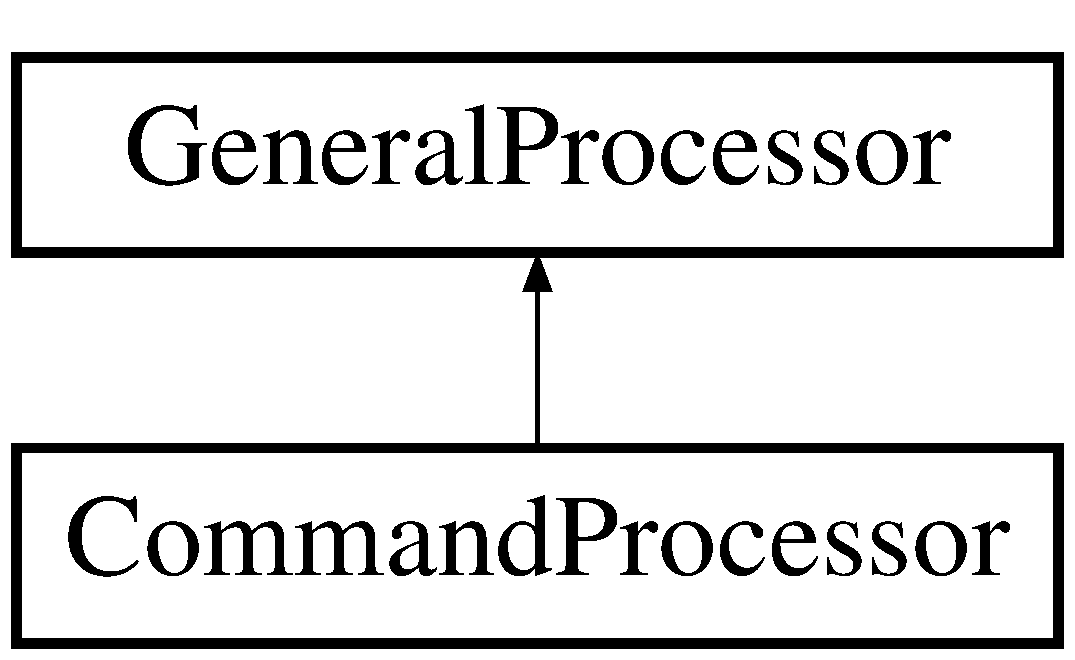
\includegraphics[height=2.000000cm]{classGeneralProcessor}
\end{center}
\end{figure}
\subsection*{Public Member Functions}
\begin{DoxyCompactItemize}
\item 
\hypertarget{classGeneralProcessor_ae1eda776118e36f2062b1f16218e0cd8}{{\bfseries General\-Processor} (int verbose=0)}\label{classGeneralProcessor_ae1eda776118e36f2062b1f16218e0cd8}

\item 
\hypertarget{classGeneralProcessor_ac25327015ff4e08b1b195e08ca5c551e}{virtual std\-::vector$<$ std\-::string $>$ {\bfseries get\-Processed\-Output} ()}\label{classGeneralProcessor_ac25327015ff4e08b1b195e08ca5c551e}

\item 
\hypertarget{classGeneralProcessor_a4c33230d64d783e11925bb99ef4d3241}{virtual bool {\bfseries is\-Ready\-To\-Process} () const }\label{classGeneralProcessor_a4c33230d64d783e11925bb99ef4d3241}

\item 
\hypertarget{classGeneralProcessor_a676b026a03d5ba50da13d7be5eacd74a}{void {\bfseries set\-Verbose} (int verbose\-Level)}\label{classGeneralProcessor_a676b026a03d5ba50da13d7be5eacd74a}

\item 
\hypertarget{classGeneralProcessor_aa5b84927347553a13167bf49cf69be8e}{virtual int {\bfseries get\-Period} () const }\label{classGeneralProcessor_aa5b84927347553a13167bf49cf69be8e}

\item 
\hypertarget{classGeneralProcessor_ae57c2ab2c7cc2a67fd535d388c39e3de}{virtual void {\bfseries set\-Period} (int new\-Period)}\label{classGeneralProcessor_ae57c2ab2c7cc2a67fd535d388c39e3de}

\end{DoxyCompactItemize}
\subsection*{Protected Attributes}
\begin{DoxyCompactItemize}
\item 
\hypertarget{classGeneralProcessor_ade0b12d7fec2b58a9782559734b00012}{int {\bfseries verbose}}\label{classGeneralProcessor_ade0b12d7fec2b58a9782559734b00012}

\item 
\hypertarget{classGeneralProcessor_a064234fe7c1400b0be5247db444367d1}{int {\bfseries period}}\label{classGeneralProcessor_a064234fe7c1400b0be5247db444367d1}

\end{DoxyCompactItemize}


The documentation for this class was generated from the following files\-:\begin{DoxyCompactItemize}
\item 
processors/General\-Processor.\-h\item 
processors/General\-Processor.\-cpp\end{DoxyCompactItemize}

\hypertarget{classGeneralProcessorFactory}{}\doxysection{General\+Processor\+Factory Class Reference}
\label{classGeneralProcessorFactory}\index{GeneralProcessorFactory@{GeneralProcessorFactory}}


A factory class for creating instances of \mbox{\hyperlink{classGeneralProcessor}{General\+Processor}}.  




{\ttfamily \#include $<$General\+Processor\+Factory.\+h$>$}

\doxysubsection*{Public Member Functions}
\begin{DoxyCompactItemize}
\item 
void \mbox{\hyperlink{classGeneralProcessorFactory_a37a1c08e8e76f05197d179a3c29f494c}{Register\+Processor}} (const std\+::string \&processor\+Type, std\+::function$<$ \mbox{\hyperlink{classGeneralProcessor}{General\+Processor}} $\ast$()$>$ creator)
\begin{DoxyCompactList}\small\item\em Registers a processor type with its creator function. \end{DoxyCompactList}\item 
\mbox{\hyperlink{classGeneralProcessor}{General\+Processor}} $\ast$ \mbox{\hyperlink{classGeneralProcessorFactory_a72e8ec568ec2d98f183681ebad80e800}{Create\+Processor}} (const std\+::string \&processor\+Type) const
\begin{DoxyCompactList}\small\item\em Creates an instance of \mbox{\hyperlink{classGeneralProcessor}{General\+Processor}} based on the provided processor type. \end{DoxyCompactList}\end{DoxyCompactItemize}
\doxysubsection*{Static Public Member Functions}
\begin{DoxyCompactItemize}
\item 
static \mbox{\hyperlink{classGeneralProcessorFactory}{General\+Processor\+Factory}} \& \mbox{\hyperlink{classGeneralProcessorFactory_a765e196b59f2a197ec9776cb51465359}{Instance}} ()
\begin{DoxyCompactList}\small\item\em Gets the singleton instance of \mbox{\hyperlink{classGeneralProcessorFactory}{General\+Processor\+Factory}}. \end{DoxyCompactList}\end{DoxyCompactItemize}


\doxysubsection{Detailed Description}
A factory class for creating instances of \mbox{\hyperlink{classGeneralProcessor}{General\+Processor}}. 

The {\ttfamily \mbox{\hyperlink{classGeneralProcessorFactory}{General\+Processor\+Factory}}} class provides functionality to register and create instances of the \mbox{\hyperlink{classGeneralProcessor}{General\+Processor}} class using a factory pattern. 

\doxysubsection{Member Function Documentation}
\mbox{\Hypertarget{classGeneralProcessorFactory_a72e8ec568ec2d98f183681ebad80e800}\label{classGeneralProcessorFactory_a72e8ec568ec2d98f183681ebad80e800}} 
\index{GeneralProcessorFactory@{GeneralProcessorFactory}!CreateProcessor@{CreateProcessor}}
\index{CreateProcessor@{CreateProcessor}!GeneralProcessorFactory@{GeneralProcessorFactory}}
\doxysubsubsection{\texorpdfstring{CreateProcessor()}{CreateProcessor()}}
{\footnotesize\ttfamily \mbox{\hyperlink{classGeneralProcessor}{General\+Processor}} $\ast$ General\+Processor\+Factory\+::\+Create\+Processor (\begin{DoxyParamCaption}\item[{const std\+::string \&}]{processor\+Type }\end{DoxyParamCaption}) const}



Creates an instance of \mbox{\hyperlink{classGeneralProcessor}{General\+Processor}} based on the provided processor type. 


\begin{DoxyParams}{Parameters}
{\em processor\+Type} & The type identifier for the processor. \\
\hline
\end{DoxyParams}
\begin{DoxyReturn}{Returns}
Pointer to the created \mbox{\hyperlink{classGeneralProcessor}{General\+Processor}} instance. 
\end{DoxyReturn}
\mbox{\Hypertarget{classGeneralProcessorFactory_a765e196b59f2a197ec9776cb51465359}\label{classGeneralProcessorFactory_a765e196b59f2a197ec9776cb51465359}} 
\index{GeneralProcessorFactory@{GeneralProcessorFactory}!Instance@{Instance}}
\index{Instance@{Instance}!GeneralProcessorFactory@{GeneralProcessorFactory}}
\doxysubsubsection{\texorpdfstring{Instance()}{Instance()}}
{\footnotesize\ttfamily \mbox{\hyperlink{classGeneralProcessorFactory}{General\+Processor\+Factory}} \& General\+Processor\+Factory\+::\+Instance (\begin{DoxyParamCaption}{ }\end{DoxyParamCaption})\hspace{0.3cm}{\ttfamily [static]}}



Gets the singleton instance of \mbox{\hyperlink{classGeneralProcessorFactory}{General\+Processor\+Factory}}. 

\begin{DoxyReturn}{Returns}
Reference to the singleton instance. 
\end{DoxyReturn}
\mbox{\Hypertarget{classGeneralProcessorFactory_a37a1c08e8e76f05197d179a3c29f494c}\label{classGeneralProcessorFactory_a37a1c08e8e76f05197d179a3c29f494c}} 
\index{GeneralProcessorFactory@{GeneralProcessorFactory}!RegisterProcessor@{RegisterProcessor}}
\index{RegisterProcessor@{RegisterProcessor}!GeneralProcessorFactory@{GeneralProcessorFactory}}
\doxysubsubsection{\texorpdfstring{RegisterProcessor()}{RegisterProcessor()}}
{\footnotesize\ttfamily void General\+Processor\+Factory\+::\+Register\+Processor (\begin{DoxyParamCaption}\item[{const std\+::string \&}]{processor\+Type,  }\item[{std\+::function$<$ \mbox{\hyperlink{classGeneralProcessor}{General\+Processor}} $\ast$()$>$}]{creator }\end{DoxyParamCaption})}



Registers a processor type with its creator function. 


\begin{DoxyParams}{Parameters}
{\em processor\+Type} & The type identifier for the processor. \\
\hline
{\em creator} & The function that creates an instance of the processor. \\
\hline
\end{DoxyParams}


The documentation for this class was generated from the following files\+:\begin{DoxyCompactItemize}
\item 
processors/General\+Processor\+Factory.\+h\item 
processors/General\+Processor\+Factory.\+cpp\end{DoxyCompactItemize}

\hypertarget{classJsonManager}{}\doxysection{Json\+Manager Class Reference}
\label{classJsonManager}\index{JsonManager@{JsonManager}}


A utility class for managing JSON configurations.  




{\ttfamily \#include $<$Json\+Manager.\+h$>$}

\doxysubsection*{Public Member Functions}
\begin{DoxyCompactItemize}
\item 
\mbox{\Hypertarget{classJsonManager_a60379eeadbb62ebe5e2f60f6b4f0c3aa}\label{classJsonManager_a60379eeadbb62ebe5e2f60f6b4f0c3aa}} 
void \mbox{\hyperlink{classJsonManager_a60379eeadbb62ebe5e2f60f6b4f0c3aa}{load\+Config\+File}} ()
\begin{DoxyCompactList}\small\item\em Loads the configuration from the specified JSON file. \end{DoxyCompactList}\item 
const nlohmann\+::json \& \mbox{\hyperlink{classJsonManager_a1e3c26143e45b7869ecb44c2dd1f9b82}{get\+Config}} () const
\begin{DoxyCompactList}\small\item\em Gets the current configuration as a const reference. \end{DoxyCompactList}\end{DoxyCompactItemize}
\doxysubsection*{Static Public Member Functions}
\begin{DoxyCompactItemize}
\item 
static \mbox{\hyperlink{classJsonManager}{Json\+Manager}} \& \mbox{\hyperlink{classJsonManager_a195c89b9868a39e6dfbacd9a491617d7}{get\+Instance}} (const std\+::string \&config\+File)
\begin{DoxyCompactList}\small\item\em Gets the singleton instance of \mbox{\hyperlink{classJsonManager}{Json\+Manager}} with a specified config file. \end{DoxyCompactList}\item 
static \mbox{\hyperlink{classJsonManager}{Json\+Manager}} \& \mbox{\hyperlink{classJsonManager_a614ccaaeebd7be1f35f12657c988b887}{get\+Instance}} ()
\begin{DoxyCompactList}\small\item\em Gets the singleton instance of \mbox{\hyperlink{classJsonManager}{Json\+Manager}} with a default config file. \end{DoxyCompactList}\end{DoxyCompactItemize}


\doxysubsection{Detailed Description}
A utility class for managing JSON configurations. 

The {\ttfamily \mbox{\hyperlink{classJsonManager}{Json\+Manager}}} class provides functionality to load and retrieve JSON configurations. 

\doxysubsection{Member Function Documentation}
\mbox{\Hypertarget{classJsonManager_a1e3c26143e45b7869ecb44c2dd1f9b82}\label{classJsonManager_a1e3c26143e45b7869ecb44c2dd1f9b82}} 
\index{JsonManager@{JsonManager}!getConfig@{getConfig}}
\index{getConfig@{getConfig}!JsonManager@{JsonManager}}
\doxysubsubsection{\texorpdfstring{getConfig()}{getConfig()}}
{\footnotesize\ttfamily const nlohmann\+::json \& Json\+Manager\+::get\+Config (\begin{DoxyParamCaption}{ }\end{DoxyParamCaption}) const}



Gets the current configuration as a const reference. 

\begin{DoxyReturn}{Returns}
Const reference to the JSON configuration. 
\end{DoxyReturn}
\mbox{\Hypertarget{classJsonManager_a614ccaaeebd7be1f35f12657c988b887}\label{classJsonManager_a614ccaaeebd7be1f35f12657c988b887}} 
\index{JsonManager@{JsonManager}!getInstance@{getInstance}}
\index{getInstance@{getInstance}!JsonManager@{JsonManager}}
\doxysubsubsection{\texorpdfstring{getInstance()}{getInstance()}\hspace{0.1cm}{\footnotesize\ttfamily [1/2]}}
{\footnotesize\ttfamily \mbox{\hyperlink{classJsonManager}{Json\+Manager}} \& Json\+Manager\+::get\+Instance (\begin{DoxyParamCaption}{ }\end{DoxyParamCaption})\hspace{0.3cm}{\ttfamily [static]}}



Gets the singleton instance of \mbox{\hyperlink{classJsonManager}{Json\+Manager}} with a default config file. 

\begin{DoxyReturn}{Returns}
Reference to the singleton instance. 
\end{DoxyReturn}
\mbox{\Hypertarget{classJsonManager_a195c89b9868a39e6dfbacd9a491617d7}\label{classJsonManager_a195c89b9868a39e6dfbacd9a491617d7}} 
\index{JsonManager@{JsonManager}!getInstance@{getInstance}}
\index{getInstance@{getInstance}!JsonManager@{JsonManager}}
\doxysubsubsection{\texorpdfstring{getInstance()}{getInstance()}\hspace{0.1cm}{\footnotesize\ttfamily [2/2]}}
{\footnotesize\ttfamily \mbox{\hyperlink{classJsonManager}{Json\+Manager}} \& Json\+Manager\+::get\+Instance (\begin{DoxyParamCaption}\item[{const std\+::string \&}]{config\+File }\end{DoxyParamCaption})\hspace{0.3cm}{\ttfamily [static]}}



Gets the singleton instance of \mbox{\hyperlink{classJsonManager}{Json\+Manager}} with a specified config file. 


\begin{DoxyParams}{Parameters}
{\em config\+File} & The path to the JSON configuration file. \\
\hline
\end{DoxyParams}
\begin{DoxyReturn}{Returns}
Reference to the singleton instance. 
\end{DoxyReturn}


The documentation for this class was generated from the following files\+:\begin{DoxyCompactItemize}
\item 
utilities/Json\+Manager.\+h\item 
utilities/Json\+Manager.\+cpp\end{DoxyCompactItemize}

\hypertarget{classProjectPrinter}{}\doxysection{Project\+Printer Class Reference}
\label{classProjectPrinter}\index{ProjectPrinter@{ProjectPrinter}}


A utility class for printing messages with various configurations.  




{\ttfamily \#include $<$Project\+Printer.\+h$>$}

\doxysubsection*{Public Member Functions}
\begin{DoxyCompactItemize}
\item 
\mbox{\Hypertarget{classProjectPrinter_a183f5abae703fd1b815d41cd91435a41}\label{classProjectPrinter_a183f5abae703fd1b815d41cd91435a41}} 
\mbox{\hyperlink{classProjectPrinter_a183f5abae703fd1b815d41cd91435a41}{Project\+Printer}} ()
\begin{DoxyCompactList}\small\item\em Default constructor for \mbox{\hyperlink{classProjectPrinter}{Project\+Printer}}. \end{DoxyCompactList}\item 
\mbox{\hyperlink{classProjectPrinter_aa5410f5d9121be33a2fe14d9ed9cf4dc}{Project\+Printer}} (bool use\+Config)
\begin{DoxyCompactList}\small\item\em Constructor for \mbox{\hyperlink{classProjectPrinter}{Project\+Printer}} with configuration based on a flag. \end{DoxyCompactList}\item 
\mbox{\hyperlink{classProjectPrinter_af054624c27d14a3a853861b72a94ce9b}{Project\+Printer}} (const std\+::string \&config\+Path)
\begin{DoxyCompactList}\small\item\em Constructor for \mbox{\hyperlink{classProjectPrinter}{Project\+Printer}} with a custom configuration file. \end{DoxyCompactList}\item 
void \mbox{\hyperlink{classProjectPrinter_aeabf297e6077912cf3073333dcadbc79}{Print}} (const std\+::string \&message, int line\+Number=0, const std\+::string \&filename=\char`\"{}\char`\"{}) const
\begin{DoxyCompactList}\small\item\em Prints a message with optional line number and filename information. \end{DoxyCompactList}\item 
void \mbox{\hyperlink{classProjectPrinter_a4a76e197a556bf291031b00992db5958}{Print\+Warning}} (const std\+::string \&message, int line\+Number=0, const std\+::string \&filename=\char`\"{}\char`\"{}) const
\begin{DoxyCompactList}\small\item\em Prints a warning message with optional line number and filename information. \end{DoxyCompactList}\item 
void \mbox{\hyperlink{classProjectPrinter_ac5ac180b0c743eac754864192c5649f0}{Print\+Error}} (const std\+::string \&message, int line\+Number=0, const std\+::string \&filename=\char`\"{}\char`\"{}) const
\begin{DoxyCompactList}\small\item\em Prints an error message with optional line number and filename information. \end{DoxyCompactList}\item 
void \mbox{\hyperlink{classProjectPrinter_af6555b81b3f6e4977e15a2b856b42793}{Print\+With\+Color}} (const std\+::string \&message, const std\+::string \&status, int line\+Number, const std\+::string \&filename, const std\+::string \&color) const
\begin{DoxyCompactList}\small\item\em Prints a message with color and optional line number and filename information. \end{DoxyCompactList}\item 
std\+::string \mbox{\hyperlink{classProjectPrinter_a30a902e6af409b4ba129da38e260dfb1}{get\+Info\+Color}} () const
\begin{DoxyCompactList}\small\item\em Gets the color for information messages. \end{DoxyCompactList}\item 
std\+::string \mbox{\hyperlink{classProjectPrinter_a0c54cfbf1eee9f871dc010000308f768}{get\+Warning\+Color}} () const
\begin{DoxyCompactList}\small\item\em Gets the color for warning messages. \end{DoxyCompactList}\item 
std\+::string \mbox{\hyperlink{classProjectPrinter_a99d72ae77c9e92214101f188fc2819f0}{get\+Error\+Color}} () const
\begin{DoxyCompactList}\small\item\em Gets the color for error messages. \end{DoxyCompactList}\item 
bool \mbox{\hyperlink{classProjectPrinter_a55c6607127f672925ee4e567e024ceca}{should\+Print\+Line\+Number}} () const
\begin{DoxyCompactList}\small\item\em Checks if line numbers should be printed. \end{DoxyCompactList}\item 
std\+::string \mbox{\hyperlink{classProjectPrinter_a49b0436d4fa79f32c10961d389b4e554}{get\+Prefix}} () const
\begin{DoxyCompactList}\small\item\em Gets the prefix for printed messages. \end{DoxyCompactList}\item 
std\+::string \mbox{\hyperlink{classProjectPrinter_a39bf7ddfa5584b478c6b2d544f36beb3}{get\+Suffix}} () const
\begin{DoxyCompactList}\small\item\em Gets the suffix for printed messages. \end{DoxyCompactList}\item 
nlohmann\+::json \mbox{\hyperlink{classProjectPrinter_ae9b53be595059692dadc889514eb1439}{get\+Config}} () const
\begin{DoxyCompactList}\small\item\em Gets the configuration as a JSON object. \end{DoxyCompactList}\item 
bool \mbox{\hyperlink{classProjectPrinter_a10bc534430156464f49dc85994950f3a}{should\+Print\+Time}} () const
\begin{DoxyCompactList}\small\item\em Checks if timestamps should be printed with messages. \end{DoxyCompactList}\item 
void \mbox{\hyperlink{classProjectPrinter_aa928801da0b7f7cd682cf4ef83860905}{set\+Info\+Color}} (const std\+::string \&color)
\begin{DoxyCompactList}\small\item\em Sets the color for information messages. \end{DoxyCompactList}\item 
void \mbox{\hyperlink{classProjectPrinter_ab0758201372a45c3d27b6dacb3a9456d}{set\+Warning\+Color}} (const std\+::string \&color)
\begin{DoxyCompactList}\small\item\em Sets the color for warning messages. \end{DoxyCompactList}\item 
void \mbox{\hyperlink{classProjectPrinter_a41a33969db5df74f99878f87a5502a83}{set\+Error\+Color}} (const std\+::string \&color)
\begin{DoxyCompactList}\small\item\em Sets the color for error messages. \end{DoxyCompactList}\item 
void \mbox{\hyperlink{classProjectPrinter_af10003b5af5c5aaf500d444151103e11}{set\+Print\+Line\+Number}} (bool print\+Line\+Num)
\begin{DoxyCompactList}\small\item\em Sets whether line numbers should be printed. \end{DoxyCompactList}\item 
void \mbox{\hyperlink{classProjectPrinter_afaf17899693e0e4638d4a94e487640ad}{set\+Prefix}} (const std\+::string \&new\+Prefix)
\begin{DoxyCompactList}\small\item\em Sets the prefix for printed messages. \end{DoxyCompactList}\item 
void \mbox{\hyperlink{classProjectPrinter_a138854bd8cf95a2535a425adc4768877}{set\+Suffix}} (const std\+::string \&new\+Suffix)
\begin{DoxyCompactList}\small\item\em Sets the suffix for printed messages. \end{DoxyCompactList}\item 
void \mbox{\hyperlink{classProjectPrinter_a1dbbbe30f40f64a83ab3cec97ea9d47a}{set\+Config}} (const nlohmann\+::json \&new\+Config)
\begin{DoxyCompactList}\small\item\em Sets the configuration using a JSON object. \end{DoxyCompactList}\item 
void \mbox{\hyperlink{classProjectPrinter_a758fe582396d7abcbd6d6534e8fb94d0}{set\+Print\+Time}} (bool print\+Time)
\begin{DoxyCompactList}\small\item\em Sets whether timestamps should be printed with messages. \end{DoxyCompactList}\end{DoxyCompactItemize}


\doxysubsection{Detailed Description}
A utility class for printing messages with various configurations. 

The {\ttfamily \mbox{\hyperlink{classProjectPrinter}{Project\+Printer}}} class provides functionality to print messages with customizable colors, prefixes, suffixes, and additional information such as line numbers and timestamps. 

\doxysubsection{Constructor \& Destructor Documentation}
\mbox{\Hypertarget{classProjectPrinter_aa5410f5d9121be33a2fe14d9ed9cf4dc}\label{classProjectPrinter_aa5410f5d9121be33a2fe14d9ed9cf4dc}} 
\index{ProjectPrinter@{ProjectPrinter}!ProjectPrinter@{ProjectPrinter}}
\index{ProjectPrinter@{ProjectPrinter}!ProjectPrinter@{ProjectPrinter}}
\doxysubsubsection{\texorpdfstring{ProjectPrinter()}{ProjectPrinter()}\hspace{0.1cm}{\footnotesize\ttfamily [1/2]}}
{\footnotesize\ttfamily Project\+Printer\+::\+Project\+Printer (\begin{DoxyParamCaption}\item[{bool}]{use\+Config }\end{DoxyParamCaption})}



Constructor for \mbox{\hyperlink{classProjectPrinter}{Project\+Printer}} with configuration based on a flag. 


\begin{DoxyParams}{Parameters}
{\em use\+Config} & A flag indicating whether to use default or custom configuration. \\
\hline
\end{DoxyParams}
\mbox{\Hypertarget{classProjectPrinter_af054624c27d14a3a853861b72a94ce9b}\label{classProjectPrinter_af054624c27d14a3a853861b72a94ce9b}} 
\index{ProjectPrinter@{ProjectPrinter}!ProjectPrinter@{ProjectPrinter}}
\index{ProjectPrinter@{ProjectPrinter}!ProjectPrinter@{ProjectPrinter}}
\doxysubsubsection{\texorpdfstring{ProjectPrinter()}{ProjectPrinter()}\hspace{0.1cm}{\footnotesize\ttfamily [2/2]}}
{\footnotesize\ttfamily Project\+Printer\+::\+Project\+Printer (\begin{DoxyParamCaption}\item[{const std\+::string \&}]{config\+Path }\end{DoxyParamCaption})}



Constructor for \mbox{\hyperlink{classProjectPrinter}{Project\+Printer}} with a custom configuration file. 


\begin{DoxyParams}{Parameters}
{\em config\+Path} & The path to the custom configuration file. \\
\hline
\end{DoxyParams}


\doxysubsection{Member Function Documentation}
\mbox{\Hypertarget{classProjectPrinter_ae9b53be595059692dadc889514eb1439}\label{classProjectPrinter_ae9b53be595059692dadc889514eb1439}} 
\index{ProjectPrinter@{ProjectPrinter}!getConfig@{getConfig}}
\index{getConfig@{getConfig}!ProjectPrinter@{ProjectPrinter}}
\doxysubsubsection{\texorpdfstring{getConfig()}{getConfig()}}
{\footnotesize\ttfamily nlohmann\+::json Project\+Printer\+::get\+Config (\begin{DoxyParamCaption}{ }\end{DoxyParamCaption}) const}



Gets the configuration as a JSON object. 

\begin{DoxyReturn}{Returns}
The configuration as a JSON object. 
\end{DoxyReturn}
\mbox{\Hypertarget{classProjectPrinter_a99d72ae77c9e92214101f188fc2819f0}\label{classProjectPrinter_a99d72ae77c9e92214101f188fc2819f0}} 
\index{ProjectPrinter@{ProjectPrinter}!getErrorColor@{getErrorColor}}
\index{getErrorColor@{getErrorColor}!ProjectPrinter@{ProjectPrinter}}
\doxysubsubsection{\texorpdfstring{getErrorColor()}{getErrorColor()}}
{\footnotesize\ttfamily std\+::string Project\+Printer\+::get\+Error\+Color (\begin{DoxyParamCaption}{ }\end{DoxyParamCaption}) const}



Gets the color for error messages. 

\begin{DoxyReturn}{Returns}
The color code for error messages. 
\end{DoxyReturn}
\mbox{\Hypertarget{classProjectPrinter_a30a902e6af409b4ba129da38e260dfb1}\label{classProjectPrinter_a30a902e6af409b4ba129da38e260dfb1}} 
\index{ProjectPrinter@{ProjectPrinter}!getInfoColor@{getInfoColor}}
\index{getInfoColor@{getInfoColor}!ProjectPrinter@{ProjectPrinter}}
\doxysubsubsection{\texorpdfstring{getInfoColor()}{getInfoColor()}}
{\footnotesize\ttfamily std\+::string Project\+Printer\+::get\+Info\+Color (\begin{DoxyParamCaption}{ }\end{DoxyParamCaption}) const}



Gets the color for information messages. 

\begin{DoxyReturn}{Returns}
The color code for information messages. 
\end{DoxyReturn}
\mbox{\Hypertarget{classProjectPrinter_a49b0436d4fa79f32c10961d389b4e554}\label{classProjectPrinter_a49b0436d4fa79f32c10961d389b4e554}} 
\index{ProjectPrinter@{ProjectPrinter}!getPrefix@{getPrefix}}
\index{getPrefix@{getPrefix}!ProjectPrinter@{ProjectPrinter}}
\doxysubsubsection{\texorpdfstring{getPrefix()}{getPrefix()}}
{\footnotesize\ttfamily std\+::string Project\+Printer\+::get\+Prefix (\begin{DoxyParamCaption}{ }\end{DoxyParamCaption}) const}



Gets the prefix for printed messages. 

\begin{DoxyReturn}{Returns}
The prefix for printed messages. 
\end{DoxyReturn}
\mbox{\Hypertarget{classProjectPrinter_a39bf7ddfa5584b478c6b2d544f36beb3}\label{classProjectPrinter_a39bf7ddfa5584b478c6b2d544f36beb3}} 
\index{ProjectPrinter@{ProjectPrinter}!getSuffix@{getSuffix}}
\index{getSuffix@{getSuffix}!ProjectPrinter@{ProjectPrinter}}
\doxysubsubsection{\texorpdfstring{getSuffix()}{getSuffix()}}
{\footnotesize\ttfamily std\+::string Project\+Printer\+::get\+Suffix (\begin{DoxyParamCaption}{ }\end{DoxyParamCaption}) const}



Gets the suffix for printed messages. 

\begin{DoxyReturn}{Returns}
The suffix for printed messages. 
\end{DoxyReturn}
\mbox{\Hypertarget{classProjectPrinter_a0c54cfbf1eee9f871dc010000308f768}\label{classProjectPrinter_a0c54cfbf1eee9f871dc010000308f768}} 
\index{ProjectPrinter@{ProjectPrinter}!getWarningColor@{getWarningColor}}
\index{getWarningColor@{getWarningColor}!ProjectPrinter@{ProjectPrinter}}
\doxysubsubsection{\texorpdfstring{getWarningColor()}{getWarningColor()}}
{\footnotesize\ttfamily std\+::string Project\+Printer\+::get\+Warning\+Color (\begin{DoxyParamCaption}{ }\end{DoxyParamCaption}) const}



Gets the color for warning messages. 

\begin{DoxyReturn}{Returns}
The color code for warning messages. 
\end{DoxyReturn}
\mbox{\Hypertarget{classProjectPrinter_aeabf297e6077912cf3073333dcadbc79}\label{classProjectPrinter_aeabf297e6077912cf3073333dcadbc79}} 
\index{ProjectPrinter@{ProjectPrinter}!Print@{Print}}
\index{Print@{Print}!ProjectPrinter@{ProjectPrinter}}
\doxysubsubsection{\texorpdfstring{Print()}{Print()}}
{\footnotesize\ttfamily void Project\+Printer\+::\+Print (\begin{DoxyParamCaption}\item[{const std\+::string \&}]{message,  }\item[{int}]{line\+Number = {\ttfamily 0},  }\item[{const std\+::string \&}]{filename = {\ttfamily \char`\"{}\char`\"{}} }\end{DoxyParamCaption}) const}



Prints a message with optional line number and filename information. 


\begin{DoxyParams}{Parameters}
{\em message} & The message to be printed. \\
\hline
{\em line\+Number} & The line number information (does not print if not specified). \\
\hline
{\em filename} & The filename information (does not print if not specified). \\
\hline
\end{DoxyParams}
\mbox{\Hypertarget{classProjectPrinter_ac5ac180b0c743eac754864192c5649f0}\label{classProjectPrinter_ac5ac180b0c743eac754864192c5649f0}} 
\index{ProjectPrinter@{ProjectPrinter}!PrintError@{PrintError}}
\index{PrintError@{PrintError}!ProjectPrinter@{ProjectPrinter}}
\doxysubsubsection{\texorpdfstring{PrintError()}{PrintError()}}
{\footnotesize\ttfamily void Project\+Printer\+::\+Print\+Error (\begin{DoxyParamCaption}\item[{const std\+::string \&}]{message,  }\item[{int}]{line\+Number = {\ttfamily 0},  }\item[{const std\+::string \&}]{filename = {\ttfamily \char`\"{}\char`\"{}} }\end{DoxyParamCaption}) const}



Prints an error message with optional line number and filename information. 


\begin{DoxyParams}{Parameters}
{\em message} & The error message to be printed. \\
\hline
{\em line\+Number} & The line number information (does not print if not specified). \\
\hline
{\em filename} & The filename information (does not print if not specified). \\
\hline
\end{DoxyParams}
\mbox{\Hypertarget{classProjectPrinter_a4a76e197a556bf291031b00992db5958}\label{classProjectPrinter_a4a76e197a556bf291031b00992db5958}} 
\index{ProjectPrinter@{ProjectPrinter}!PrintWarning@{PrintWarning}}
\index{PrintWarning@{PrintWarning}!ProjectPrinter@{ProjectPrinter}}
\doxysubsubsection{\texorpdfstring{PrintWarning()}{PrintWarning()}}
{\footnotesize\ttfamily void Project\+Printer\+::\+Print\+Warning (\begin{DoxyParamCaption}\item[{const std\+::string \&}]{message,  }\item[{int}]{line\+Number = {\ttfamily 0},  }\item[{const std\+::string \&}]{filename = {\ttfamily \char`\"{}\char`\"{}} }\end{DoxyParamCaption}) const}



Prints a warning message with optional line number and filename information. 


\begin{DoxyParams}{Parameters}
{\em message} & The warning message to be printed. \\
\hline
{\em line\+Number} & The line number information (does not print if not specified). \\
\hline
{\em filename} & The filename information (does not print if not specified). \\
\hline
\end{DoxyParams}
\mbox{\Hypertarget{classProjectPrinter_af6555b81b3f6e4977e15a2b856b42793}\label{classProjectPrinter_af6555b81b3f6e4977e15a2b856b42793}} 
\index{ProjectPrinter@{ProjectPrinter}!PrintWithColor@{PrintWithColor}}
\index{PrintWithColor@{PrintWithColor}!ProjectPrinter@{ProjectPrinter}}
\doxysubsubsection{\texorpdfstring{PrintWithColor()}{PrintWithColor()}}
{\footnotesize\ttfamily void Project\+Printer\+::\+Print\+With\+Color (\begin{DoxyParamCaption}\item[{const std\+::string \&}]{message,  }\item[{const std\+::string \&}]{status,  }\item[{int}]{line\+Number,  }\item[{const std\+::string \&}]{filename,  }\item[{const std\+::string \&}]{color }\end{DoxyParamCaption}) const}



Prints a message with color and optional line number and filename information. 


\begin{DoxyParams}{Parameters}
{\em message} & The message to be printed. \\
\hline
{\em status} & The status or color of the message. \\
\hline
{\em line\+Number} & The line number information (does not print if not specified). \\
\hline
{\em filename} & The filename information (does not print if not specified). \\
\hline
{\em color} & The color code for the message (default is no color). \\
\hline
\end{DoxyParams}
\mbox{\Hypertarget{classProjectPrinter_a1dbbbe30f40f64a83ab3cec97ea9d47a}\label{classProjectPrinter_a1dbbbe30f40f64a83ab3cec97ea9d47a}} 
\index{ProjectPrinter@{ProjectPrinter}!setConfig@{setConfig}}
\index{setConfig@{setConfig}!ProjectPrinter@{ProjectPrinter}}
\doxysubsubsection{\texorpdfstring{setConfig()}{setConfig()}}
{\footnotesize\ttfamily void Project\+Printer\+::set\+Config (\begin{DoxyParamCaption}\item[{const nlohmann\+::json \&}]{new\+Config }\end{DoxyParamCaption})}



Sets the configuration using a JSON object. 


\begin{DoxyParams}{Parameters}
{\em new\+Config} & The new configuration as a JSON object. \\
\hline
\end{DoxyParams}
\mbox{\Hypertarget{classProjectPrinter_a41a33969db5df74f99878f87a5502a83}\label{classProjectPrinter_a41a33969db5df74f99878f87a5502a83}} 
\index{ProjectPrinter@{ProjectPrinter}!setErrorColor@{setErrorColor}}
\index{setErrorColor@{setErrorColor}!ProjectPrinter@{ProjectPrinter}}
\doxysubsubsection{\texorpdfstring{setErrorColor()}{setErrorColor()}}
{\footnotesize\ttfamily void Project\+Printer\+::set\+Error\+Color (\begin{DoxyParamCaption}\item[{const std\+::string \&}]{color }\end{DoxyParamCaption})}



Sets the color for error messages. 


\begin{DoxyParams}{Parameters}
{\em color} & The new color code for error messages. \\
\hline
\end{DoxyParams}
\mbox{\Hypertarget{classProjectPrinter_aa928801da0b7f7cd682cf4ef83860905}\label{classProjectPrinter_aa928801da0b7f7cd682cf4ef83860905}} 
\index{ProjectPrinter@{ProjectPrinter}!setInfoColor@{setInfoColor}}
\index{setInfoColor@{setInfoColor}!ProjectPrinter@{ProjectPrinter}}
\doxysubsubsection{\texorpdfstring{setInfoColor()}{setInfoColor()}}
{\footnotesize\ttfamily void Project\+Printer\+::set\+Info\+Color (\begin{DoxyParamCaption}\item[{const std\+::string \&}]{color }\end{DoxyParamCaption})}



Sets the color for information messages. 


\begin{DoxyParams}{Parameters}
{\em color} & The new color code for information messages. \\
\hline
\end{DoxyParams}
\mbox{\Hypertarget{classProjectPrinter_afaf17899693e0e4638d4a94e487640ad}\label{classProjectPrinter_afaf17899693e0e4638d4a94e487640ad}} 
\index{ProjectPrinter@{ProjectPrinter}!setPrefix@{setPrefix}}
\index{setPrefix@{setPrefix}!ProjectPrinter@{ProjectPrinter}}
\doxysubsubsection{\texorpdfstring{setPrefix()}{setPrefix()}}
{\footnotesize\ttfamily void Project\+Printer\+::set\+Prefix (\begin{DoxyParamCaption}\item[{const std\+::string \&}]{new\+Prefix }\end{DoxyParamCaption})}



Sets the prefix for printed messages. 


\begin{DoxyParams}{Parameters}
{\em new\+Prefix} & The new prefix for printed messages. \\
\hline
\end{DoxyParams}
\mbox{\Hypertarget{classProjectPrinter_af10003b5af5c5aaf500d444151103e11}\label{classProjectPrinter_af10003b5af5c5aaf500d444151103e11}} 
\index{ProjectPrinter@{ProjectPrinter}!setPrintLineNumber@{setPrintLineNumber}}
\index{setPrintLineNumber@{setPrintLineNumber}!ProjectPrinter@{ProjectPrinter}}
\doxysubsubsection{\texorpdfstring{setPrintLineNumber()}{setPrintLineNumber()}}
{\footnotesize\ttfamily void Project\+Printer\+::set\+Print\+Line\+Number (\begin{DoxyParamCaption}\item[{bool}]{print\+Line\+Num }\end{DoxyParamCaption})}



Sets whether line numbers should be printed. 


\begin{DoxyParams}{Parameters}
{\em print\+Line\+Num} & True to print line numbers, false otherwise. \\
\hline
\end{DoxyParams}
\mbox{\Hypertarget{classProjectPrinter_a758fe582396d7abcbd6d6534e8fb94d0}\label{classProjectPrinter_a758fe582396d7abcbd6d6534e8fb94d0}} 
\index{ProjectPrinter@{ProjectPrinter}!setPrintTime@{setPrintTime}}
\index{setPrintTime@{setPrintTime}!ProjectPrinter@{ProjectPrinter}}
\doxysubsubsection{\texorpdfstring{setPrintTime()}{setPrintTime()}}
{\footnotesize\ttfamily void Project\+Printer\+::set\+Print\+Time (\begin{DoxyParamCaption}\item[{bool}]{print\+Time }\end{DoxyParamCaption})}



Sets whether timestamps should be printed with messages. 


\begin{DoxyParams}{Parameters}
{\em print\+Time} & True to print timestamps, false otherwise. \\
\hline
\end{DoxyParams}
\mbox{\Hypertarget{classProjectPrinter_a138854bd8cf95a2535a425adc4768877}\label{classProjectPrinter_a138854bd8cf95a2535a425adc4768877}} 
\index{ProjectPrinter@{ProjectPrinter}!setSuffix@{setSuffix}}
\index{setSuffix@{setSuffix}!ProjectPrinter@{ProjectPrinter}}
\doxysubsubsection{\texorpdfstring{setSuffix()}{setSuffix()}}
{\footnotesize\ttfamily void Project\+Printer\+::set\+Suffix (\begin{DoxyParamCaption}\item[{const std\+::string \&}]{new\+Suffix }\end{DoxyParamCaption})}



Sets the suffix for printed messages. 


\begin{DoxyParams}{Parameters}
{\em new\+Suffix} & The new suffix for printed messages. \\
\hline
\end{DoxyParams}
\mbox{\Hypertarget{classProjectPrinter_ab0758201372a45c3d27b6dacb3a9456d}\label{classProjectPrinter_ab0758201372a45c3d27b6dacb3a9456d}} 
\index{ProjectPrinter@{ProjectPrinter}!setWarningColor@{setWarningColor}}
\index{setWarningColor@{setWarningColor}!ProjectPrinter@{ProjectPrinter}}
\doxysubsubsection{\texorpdfstring{setWarningColor()}{setWarningColor()}}
{\footnotesize\ttfamily void Project\+Printer\+::set\+Warning\+Color (\begin{DoxyParamCaption}\item[{const std\+::string \&}]{color }\end{DoxyParamCaption})}



Sets the color for warning messages. 


\begin{DoxyParams}{Parameters}
{\em color} & The new color code for warning messages. \\
\hline
\end{DoxyParams}
\mbox{\Hypertarget{classProjectPrinter_a55c6607127f672925ee4e567e024ceca}\label{classProjectPrinter_a55c6607127f672925ee4e567e024ceca}} 
\index{ProjectPrinter@{ProjectPrinter}!shouldPrintLineNumber@{shouldPrintLineNumber}}
\index{shouldPrintLineNumber@{shouldPrintLineNumber}!ProjectPrinter@{ProjectPrinter}}
\doxysubsubsection{\texorpdfstring{shouldPrintLineNumber()}{shouldPrintLineNumber()}}
{\footnotesize\ttfamily bool Project\+Printer\+::should\+Print\+Line\+Number (\begin{DoxyParamCaption}{ }\end{DoxyParamCaption}) const}



Checks if line numbers should be printed. 

\begin{DoxyReturn}{Returns}
True if line numbers should be printed, false otherwise. 
\end{DoxyReturn}
\mbox{\Hypertarget{classProjectPrinter_a10bc534430156464f49dc85994950f3a}\label{classProjectPrinter_a10bc534430156464f49dc85994950f3a}} 
\index{ProjectPrinter@{ProjectPrinter}!shouldPrintTime@{shouldPrintTime}}
\index{shouldPrintTime@{shouldPrintTime}!ProjectPrinter@{ProjectPrinter}}
\doxysubsubsection{\texorpdfstring{shouldPrintTime()}{shouldPrintTime()}}
{\footnotesize\ttfamily bool Project\+Printer\+::should\+Print\+Time (\begin{DoxyParamCaption}{ }\end{DoxyParamCaption}) const}



Checks if timestamps should be printed with messages. 

\begin{DoxyReturn}{Returns}
True if timestamps should be printed, false otherwise. 
\end{DoxyReturn}


The documentation for this class was generated from the following files\+:\begin{DoxyCompactItemize}
\item 
utilities/Project\+Printer.\+h\item 
utilities/Project\+Printer.\+cpp\end{DoxyCompactItemize}

\hypertarget{classSignalHandler}{}\doxysection{Signal\+Handler Class Reference}
\label{classSignalHandler}\index{SignalHandler@{SignalHandler}}


A class to handle signals, such as interrupt signals (Ctrl+C) and termination signals.  




{\ttfamily \#include $<$Signal\+Handler.\+h$>$}

\doxysubsection*{Public Member Functions}
\begin{DoxyCompactItemize}
\item 
\mbox{\Hypertarget{classSignalHandler_a3149ab1b5e1c8940d11b182f8059d916}\label{classSignalHandler_a3149ab1b5e1c8940d11b182f8059d916}} 
\mbox{\hyperlink{classSignalHandler_a3149ab1b5e1c8940d11b182f8059d916}{Signal\+Handler}} ()
\begin{DoxyCompactList}\small\item\em Constructor for \mbox{\hyperlink{classSignalHandler}{Signal\+Handler}}. \end{DoxyCompactList}\item 
\mbox{\hyperlink{classSignalHandler_addc8b5b0b969eb405376a77a369de007}{$\sim$\+Signal\+Handler}} ()
\begin{DoxyCompactList}\small\item\em Destructor for \mbox{\hyperlink{classSignalHandler}{Signal\+Handler}}. \end{DoxyCompactList}\item 
bool \mbox{\hyperlink{classSignalHandler_a4f725f94ab6c769eef1ca03d8b561473}{is\+Quit\+Signal\+Received}} () const
\begin{DoxyCompactList}\small\item\em Checks whether a quit signal is received. \end{DoxyCompactList}\end{DoxyCompactItemize}
\doxysubsection*{Static Public Member Functions}
\begin{DoxyCompactItemize}
\item 
static \mbox{\hyperlink{classSignalHandler}{Signal\+Handler}} \& \mbox{\hyperlink{classSignalHandler_a15631110fc9c8fee4c1b2bf3bced2de3}{get\+Instance}} ()
\begin{DoxyCompactList}\small\item\em Static function to get the singleton instance of \mbox{\hyperlink{classSignalHandler}{Signal\+Handler}}. \end{DoxyCompactList}\end{DoxyCompactItemize}


\doxysubsection{Detailed Description}
A class to handle signals, such as interrupt signals (Ctrl+C) and termination signals. 

The {\ttfamily \mbox{\hyperlink{classSignalHandler}{Signal\+Handler}}} class provides functionality to handle signals and determine whether a quit signal is received. 

\doxysubsection{Constructor \& Destructor Documentation}
\mbox{\Hypertarget{classSignalHandler_addc8b5b0b969eb405376a77a369de007}\label{classSignalHandler_addc8b5b0b969eb405376a77a369de007}} 
\index{SignalHandler@{SignalHandler}!````~SignalHandler@{$\sim$SignalHandler}}
\index{````~SignalHandler@{$\sim$SignalHandler}!SignalHandler@{SignalHandler}}
\doxysubsubsection{\texorpdfstring{$\sim$SignalHandler()}{~SignalHandler()}}
{\footnotesize\ttfamily Signal\+Handler\+::$\sim$\+Signal\+Handler (\begin{DoxyParamCaption}{ }\end{DoxyParamCaption})}



Destructor for \mbox{\hyperlink{classSignalHandler}{Signal\+Handler}}. 

Unregisters signal handlers during destruction. 

\doxysubsection{Member Function Documentation}
\mbox{\Hypertarget{classSignalHandler_a15631110fc9c8fee4c1b2bf3bced2de3}\label{classSignalHandler_a15631110fc9c8fee4c1b2bf3bced2de3}} 
\index{SignalHandler@{SignalHandler}!getInstance@{getInstance}}
\index{getInstance@{getInstance}!SignalHandler@{SignalHandler}}
\doxysubsubsection{\texorpdfstring{getInstance()}{getInstance()}}
{\footnotesize\ttfamily \mbox{\hyperlink{classSignalHandler}{Signal\+Handler}} \& Signal\+Handler\+::get\+Instance (\begin{DoxyParamCaption}{ }\end{DoxyParamCaption})\hspace{0.3cm}{\ttfamily [static]}}



Static function to get the singleton instance of \mbox{\hyperlink{classSignalHandler}{Signal\+Handler}}. 

\begin{DoxyReturn}{Returns}
Reference to the singleton instance. 
\end{DoxyReturn}
\mbox{\Hypertarget{classSignalHandler_a4f725f94ab6c769eef1ca03d8b561473}\label{classSignalHandler_a4f725f94ab6c769eef1ca03d8b561473}} 
\index{SignalHandler@{SignalHandler}!isQuitSignalReceived@{isQuitSignalReceived}}
\index{isQuitSignalReceived@{isQuitSignalReceived}!SignalHandler@{SignalHandler}}
\doxysubsubsection{\texorpdfstring{isQuitSignalReceived()}{isQuitSignalReceived()}}
{\footnotesize\ttfamily bool Signal\+Handler\+::is\+Quit\+Signal\+Received (\begin{DoxyParamCaption}{ }\end{DoxyParamCaption}) const}



Checks whether a quit signal is received. 

\begin{DoxyReturn}{Returns}
True if a quit signal is received, false otherwise. 
\end{DoxyReturn}


The documentation for this class was generated from the following files\+:\begin{DoxyCompactItemize}
\item 
utilities/Signal\+Handler.\+h\item 
utilities/Signal\+Handler.\+cpp\end{DoxyCompactItemize}

\hypertarget{classTypeChecker}{}\doxysection{Type\+Checker Class Reference}
\label{classTypeChecker}\index{TypeChecker@{TypeChecker}}


A utility class for type checking.  




{\ttfamily \#include $<$Type\+Checker.\+h$>$}

\doxysubsection*{Static Public Member Functions}
\begin{DoxyCompactItemize}
\item 
{\footnotesize template$<$typename Base , typename Derived $>$ }\\static bool \mbox{\hyperlink{classTypeChecker_a0a0d73da592a8598bf316b55e7d94efe}{Is\+Instance\+Of}} (const Derived $\ast$derived\+Ptr)
\begin{DoxyCompactList}\small\item\em Checks if a pointer is an instance of a specific base type. \end{DoxyCompactList}\item 
{\footnotesize template$<$typename Base , typename Derived $>$ }\\static bool \mbox{\hyperlink{classTypeChecker_a9a7b060e6f33fce02cc87a70f36ec0b1}{Is\+Instance\+Of}} (const std\+::shared\+\_\+ptr$<$ Derived $>$ \&derived\+Ptr)
\begin{DoxyCompactList}\small\item\em Checks if a shared pointer is an instance of a specific base type. \end{DoxyCompactList}\end{DoxyCompactItemize}


\doxysubsection{Detailed Description}
A utility class for type checking. 

The {\ttfamily \mbox{\hyperlink{classTypeChecker}{Type\+Checker}}} class provides template-\/based methods for checking whether an object or a smart pointer is an instance of a certain base type. 

\doxysubsection{Member Function Documentation}
\mbox{\Hypertarget{classTypeChecker_a0a0d73da592a8598bf316b55e7d94efe}\label{classTypeChecker_a0a0d73da592a8598bf316b55e7d94efe}} 
\index{TypeChecker@{TypeChecker}!IsInstanceOf@{IsInstanceOf}}
\index{IsInstanceOf@{IsInstanceOf}!TypeChecker@{TypeChecker}}
\doxysubsubsection{\texorpdfstring{IsInstanceOf()}{IsInstanceOf()}\hspace{0.1cm}{\footnotesize\ttfamily [1/2]}}
{\footnotesize\ttfamily template$<$typename Base , typename Derived $>$ \\
static bool Type\+Checker\+::\+Is\+Instance\+Of (\begin{DoxyParamCaption}\item[{const Derived $\ast$}]{derived\+Ptr }\end{DoxyParamCaption})\hspace{0.3cm}{\ttfamily [inline]}, {\ttfamily [static]}}



Checks if a pointer is an instance of a specific base type. 


\begin{DoxyTemplParams}{Template Parameters}
{\em Base} & The base type. \\
\hline
{\em Derived} & The derived type. \\
\hline
\end{DoxyTemplParams}

\begin{DoxyParams}{Parameters}
{\em derived\+Ptr} & Pointer to the derived type. \\
\hline
\end{DoxyParams}
\begin{DoxyReturn}{Returns}
True if the pointer is an instance of the base type, false otherwise. 
\end{DoxyReturn}
\mbox{\Hypertarget{classTypeChecker_a9a7b060e6f33fce02cc87a70f36ec0b1}\label{classTypeChecker_a9a7b060e6f33fce02cc87a70f36ec0b1}} 
\index{TypeChecker@{TypeChecker}!IsInstanceOf@{IsInstanceOf}}
\index{IsInstanceOf@{IsInstanceOf}!TypeChecker@{TypeChecker}}
\doxysubsubsection{\texorpdfstring{IsInstanceOf()}{IsInstanceOf()}\hspace{0.1cm}{\footnotesize\ttfamily [2/2]}}
{\footnotesize\ttfamily template$<$typename Base , typename Derived $>$ \\
static bool Type\+Checker\+::\+Is\+Instance\+Of (\begin{DoxyParamCaption}\item[{const std\+::shared\+\_\+ptr$<$ Derived $>$ \&}]{derived\+Ptr }\end{DoxyParamCaption})\hspace{0.3cm}{\ttfamily [inline]}, {\ttfamily [static]}}



Checks if a shared pointer is an instance of a specific base type. 


\begin{DoxyTemplParams}{Template Parameters}
{\em Base} & The base type. \\
\hline
{\em Derived} & The derived type. \\
\hline
\end{DoxyTemplParams}

\begin{DoxyParams}{Parameters}
{\em derived\+Ptr} & Shared pointer to the derived type. \\
\hline
\end{DoxyParams}
\begin{DoxyReturn}{Returns}
True if the shared pointer is an instance of the base type, false otherwise. 
\end{DoxyReturn}


The documentation for this class was generated from the following file\+:\begin{DoxyCompactItemize}
\item 
utilities/Type\+Checker.\+h\end{DoxyCompactItemize}

\chapter{File Documentation}
\hypertarget{main_8cpp}{}\doxysection{main.\+cpp File Reference}
\label{main_8cpp}\index{main.cpp@{main.cpp}}


Entry point for the program.  


{\ttfamily \#include \char`\"{}Project\+Printer.\+h\char`\"{}}\newline
{\ttfamily \#include \char`\"{}Json\+Manager.\+h\char`\"{}}\newline
{\ttfamily \#include \char`\"{}Data\+Transmitter\+Manager.\+h\char`\"{}}\newline
{\ttfamily \#include \char`\"{}Data\+Channel\+Manager.\+h\char`\"{}}\newline
{\ttfamily \#include \char`\"{}Signal\+Handler.\+h\char`\"{}}\newline
{\ttfamily \#include \char`\"{}General\+Processor\+Factory.\+h\char`\"{}}\newline
{\ttfamily \#include \char`\"{}General\+Processor.\+h\char`\"{}}\newline
{\ttfamily \#include \char`\"{}Command\+Processor.\+h\char`\"{}}\newline
{\ttfamily \#include $<$nlohmann/json.\+hpp$>$}\newline
{\ttfamily \#include $<$fstream$>$}\newline
{\ttfamily \#include $<$chrono$>$}\newline
{\ttfamily \#include $<$thread$>$}\newline
\doxysubsection*{Typedefs}
\begin{DoxyCompactItemize}
\item 
\mbox{\Hypertarget{main_8cpp_ab701e3ac61a85b337ec5c1abaad6742d}\label{main_8cpp_ab701e3ac61a85b337ec5c1abaad6742d}} 
using {\bfseries json} = nlohmann\+::json
\end{DoxyCompactItemize}
\doxysubsection*{Functions}
\begin{DoxyCompactItemize}
\item 
void \mbox{\hyperlink{main_8cpp_abc6bfde2d5a3c8cd29cae7c4c0675129}{register\+Processors}} (nlohmann\+::json config)
\begin{DoxyCompactList}\small\item\em Function to register processor classes. \end{DoxyCompactList}\item 
int \mbox{\hyperlink{main_8cpp_a0ddf1224851353fc92bfbff6f499fa97}{main}} (int argc, char $\ast$argv\mbox{[}$\,$\mbox{]})
\begin{DoxyCompactList}\small\item\em The main function of the program. \end{DoxyCompactList}\end{DoxyCompactItemize}


\doxysubsection{Detailed Description}
Entry point for the program. 



\doxysubsection{Function Documentation}
\mbox{\Hypertarget{main_8cpp_a0ddf1224851353fc92bfbff6f499fa97}\label{main_8cpp_a0ddf1224851353fc92bfbff6f499fa97}} 
\index{main.cpp@{main.cpp}!main@{main}}
\index{main@{main}!main.cpp@{main.cpp}}
\doxysubsubsection{\texorpdfstring{main()}{main()}}
{\footnotesize\ttfamily int main (\begin{DoxyParamCaption}\item[{int}]{argc,  }\item[{char $\ast$}]{argv\mbox{[}$\,$\mbox{]} }\end{DoxyParamCaption})}



The main function of the program. 


\begin{DoxyParams}{Parameters}
{\em argc} & Number of command-\/line arguments. \\
\hline
{\em argv} & Array of command-\/line arguments. \\
\hline
\end{DoxyParams}
\begin{DoxyReturn}{Returns}
Exit code. 
\end{DoxyReturn}
\mbox{\Hypertarget{main_8cpp_abc6bfde2d5a3c8cd29cae7c4c0675129}\label{main_8cpp_abc6bfde2d5a3c8cd29cae7c4c0675129}} 
\index{main.cpp@{main.cpp}!registerProcessors@{registerProcessors}}
\index{registerProcessors@{registerProcessors}!main.cpp@{main.cpp}}
\doxysubsubsection{\texorpdfstring{registerProcessors()}{registerProcessors()}}
{\footnotesize\ttfamily void register\+Processors (\begin{DoxyParamCaption}\item[{nlohmann\+::json}]{config }\end{DoxyParamCaption})}



Function to register processor classes. 

New processors MUST be registered here!


\begin{DoxyParams}{Parameters}
{\em config} & Configuration data in JSON format. \\
\hline
\end{DoxyParams}

%--- End generated contents ---

% Index
\newpage
\phantomsection
\addcontentsline{toc}{part}{Index}
\printindex

\end{document}
